\documentclass{article}
\usepackage{graphicx}
\usepackage{multicol}
\usepackage{amsmath}
\usepackage{tcolorbox}
\usepackage{subcaption}
\usepackage[spanish]{babel}
\usepackage{lipsum}

\title{Reconocimiento de señales de tráfico en Cuba}
\author {
Claudia Alvarez Martínez \and
Roger Moreno Gutiérrez \and
Kevin Majim Ortega Alvarez \and
Jan Carlos Perez González
}

\date {\today}

\begin{document}
\begin{figure}[t]
    \centering
    
\includegraphics{resources/logo matcompng.png}
\end{figure}
\maketitle
\begin{center}
Facultad de Matemática y Computación.

 Universidad de la Habana
\end{center}
\newpage
\begin{abstract}
La detección y clasificación de señales de tránsito es una tarea para apoyar al conductor e incluso asistir en la navegación de un automóvil autónomo. El objetivo de este trabajo es presentar una metodología para la detección y clasificación de señales de tráfico cubanas mediante el uso de redes convolucionales. La metodología se divide en cinco etapas, 1-) se realiza la recolección de 615 de señales de tráfico en un ambiente no controlado, 2-) se realiza un proceso manual de marcado para la detección de señales de tráfico en las imágenes, 3-) se entrena una red neuronal (YOLOv8) en el conjunto GTSRB para obtener un conocimiento general de las características de las señales, 4-) se evalúa esa red neuronal en el conjunto de datos creado, 5-) se realiza un proceso de transferencia de conocimiento y aumentado de datos para la clasificación. De acuerdo con los resultados obtenidos de los experimentos se concluye que la metodología propuesta permite reconocer señales de tráfico cubanas con un \textit{mAP@0.5} del $75\%$, sin embargo tras la experimentación con filmaciones en tiempo real, se obtienen mejores resultados.
\vfill
\textbf{Palabras clave}: Señales de tráfico, redes convolucionales, imágenes segmentadas, YOLOv8
\end{abstract}
\newpage


%=========================INTRODUCCION=================================


\section{Introducción}
Las señales de tráfico son los signos visuales utilizados para ofrecerle información a los conductores y peatones que transitan por un camino. Las señales de tráfico se clasifican de acuerdo a sus colores y formas, de manera que sean llamativas para que los automovilistas les presten atención. Muchos países europeos han trabajado para estandarizar las señales de tráfico, lo que dio lugar a la convención de Viena del 8 de noviembre de 1968. 

Particularmente en nuestro país, las señales de tránsito se distribuyen en 8 grupos\cite{ref7}, entre las que se encuentran algunas de prohibición, que por lo general son blancas y rojas en los bordes, las de peligro son triángulos amarillos o las de obligación que son redondas y de fondo azul.
\subsection{Motivación}
Es ampliamente reconocido por todos los conductores la importancia de obedecer las leyes de tránsito, prestando especial atención a las señales de tráfico. Las consecuencias de no hacerlo pueden ser desastrosas, especialmente cuando estas señales se encuentran en mal estado debido a las inclemencias del clima, la mala iluminación, o simplemente no se ven a tiempo. Por ello, es crucial desarrollar un sistema automatizado que pueda detectar de forma rápida y eficiente estas señales. Además, este sistema puede ser utilizado como asistencia a conductores, mejorando significativamente la seguridad en las vías.
\subsection{Problemática}
A pesar de los avances en la tecnología de reconocimiento de imágenes, el diseño de un sistema de detección de señales de tráfico que funcione de manera confiable en diversas condiciones sigue siendo un desafío. Las señales de tráfico pueden verse afectadas por múltiples factores, como la variabilidad en la iluminación, las condiciones climáticas adversas, la obstrucción parcial por otros objetos y el desgaste físico. Además, las señales pueden variar significativamente en apariencia dependiendo de la región o país, lo que complica aún más la tarea de desarrollar un sistema universalmente eficaz. En el contexto específico de Cuba, la diversidad de señales y su estado de conservación presenta un desafío adicional para la implementación de estos sistemas.
\subsection{Objetivos generales y específicos}
\textbf{Objetivo General:} Desarrollar una metodología para la detección y clasificación de señales de tráfico cubanas utilizando técnicas avanzadas de reconocimiento de imágenes, además de proporcionar una base de datos de señales obtenidas en un entorno no controlado para la evaluación y mejora de los modelos de detección.
\newpage
\textbf{Objetivos Específicos:}
\begin{itemize}
    \item{Crear una base de datos: Recopilar y etiquetar imágenes de señales de tráfico cubanas en diferentes condiciones ambientales y de iluminación.}
    \item{Desarrollar un algoritmo de detección: Entrenar un modelo de aprendizaje automático que pueda detectar y clasificar señales de tráfico con alta precisión.}
    \item{Evaluar el desempeño del modelo: Probar el modelo en escenarios reales y comparar su rendimiento con métodos existentes.}
    \item{Mejorar la robustez del sistema: Investigar y aplicar técnicas para mejorar la resistencia del sistema a variaciones en la iluminación y las condiciones climáticas adversas.}
\end{itemize}
\newpage


%================================ESTADO DEL ARTE ==============================================


\section{Revisión bibliográfica}
Dado que las señales de tráfico se clasifican por sus formas y colores, se pueden aplicar técnicas de aprendizaje de máquinas y visión computacional para su reconocimiento \cite{ref6}, aunque las más utilizadas son las redes convolucionales pues estas han demostrado poseer una gran precisión en la detección de señales. A. Hechri y A. Mtibaa \cite{ref8} realizan una comparación entre dos aproximaciones distintas, una utilizando Maquinas de Soporte Vectorial (SVM por sus siglas en inglés) y la otra utilizando redes convolucionales, además proponen un nuevo modelo a dos fases, la primera de detección y reconocimiento, en la cual utilizan el SVM, y la segunda de clasificación, en la cual utiliza redes convolucionales para esta tarea. Se muestran resultados prometedores para este modelo, y un tanto desalentadores para el SVM.

Divya Elankumaran \cite{ref5} propone un algoritmo que combina redes residuales (ResNet-50), YOLOv8 (You Only Look Once) y redes neuronales convolucionales profundas (DCNN) durante el entrenamiento para resolver esta tarea. En él, se utiliza YOLOv8 para la detección de las señales, mientras que de la clasificación se utilizan las DCNN, y para mitigar el efecto que pueda tener el trabajo con estas redes profundas se utiliza ResNet-50, dado que como posee capas residuales, permite que el gradiente salte ciertas capas durante el entrenamiento.

Gege Guo y Zhenyu Zhang \cite{ref9} crean un algoritmo ligero basado en YOLOv5s para la detección de baches en las calles de manera más rápida, y aunque no detecte señales de tránsito, utiliza varias técnicas que son interesantes. Cambian la estructura de YOLOv5s, dado que modifican la columna (Backbone) del mismo utilizando una red MobileNetV3, la cual es una red, eficiente en términos de computación y memoria, lo cual se traduce en una mayor rapidez, aplican el algoritmo de KMeans para determinar automáticamente las mejores anclas ("anchor boxes" son uno de los hiperparámetros de YOLOv5); el suavizado de etiquetas y la reparametrización estructural. en el año 2022, Yanzhao Zhu y Wei Qi Yan \cite{ref1} realizan una comparación entre los modelos de YOLOv5 y SSD (Single Shot MultiBox Detector), donde los resultados evidencian que YOLOv5 posee métricas mejores para el reconocimiento de señales.


En 2023 Weizhen Song and Shahrel Azmin Suani\cite{ref2} proponen un nuevo modelo basado en YOLOv4-tiny y que utiliza una versión simplificada CSPDarknet53 para la extracción de características, Agrupamiento de Pirámides Espaciales Mejorado (spatial-pyramid-pooling) lo cual mejora la capacidad del modelo para procesar objetos de diferentes tamaños; además de utilizar el algoritmo e K-Means para agrupar los datos y encontrar las mejores cajas anclas (anchor boxes).

Para concluir, los métodos basados en aprendizaje profundo, nos ofrecen amplios beneficios, dado su efectividad, precisión y rapidez para detectar y clasificar señales. En particular YOLO, es el que mejores resultados ofrece, además con la llegada de YOLOv8, como son la optimización de bloques residuales y cuellos de botella (\textit{bottleneck blocks}) más eficientes, optimización de anclas con el algoritmo de \textit{K-Means++} mejorando la precisión del modelo, se han mejorado las partes fundamentales de la red (\textit{backbone}) y la cabeza de la red (\textit{head}) para una mejor extracción de características y detección de objetos; hace que YOLOv8 sea un buen candidato para utilizar en nuestro modelo.

\begin{tcolorbox}
En el archivo \textit{state\_of\_art/state\_of\_art.html} se recoge un resumen de las revisiones bibliográficas que se hicieron
\end{tcolorbox}

%================================MODELO PARTE 1=======================================


\section{Nuestro Modelo}
Para una mejor comprensión de la solución, vamos dividir el capítulo en 6 temas fundamentales.\\
\begin{itemize}
\item{\textbf{Línea de trabajo:} Se abordará una explicación general del enfoque de la solución, definiendo todos los procesos que se completaron en la misma.}
\item{\textbf{Conjuntos de datos:} Explicaremos el proceso de obtención y procesamiento de los datos que se utilizaron para la solución.}
\item{\textbf{Entrenamiento, validación y evaluación:} Abordaremos el proceso de entrenamiento de los diferentes modelos utilizados y se explicarán los resultados obtenidos de los modelos a partir de los datos de validación y evaluación.}
\item{\textbf{Pruebas de campo:} Mostraremos resultados de los modelos en las pruebas de campo.}
\end{itemize}
\subsection{Línea de trabajo}
El enfoque principal consiste en clasificar las señales de tráfico en una de las siguientes cuatro categorías fundamentales: 
\begin{itemize}
\item{Prohibición}
\item{Peligro}
\item{Obligación}
\item{Otra}
\end{itemize}
Para lograr esto, hemos optado por el modelo \textbf{YOLOv8n}, dado que frente a las limitaciones de cómputo, es una alternativa ligera, además de su capacidad para mantener un equilibrio óptimo entre velocidad de procesamiento y precisión. Este modelo, previamente entrenado en un conjunto diverso de imágenes, será reentrenado específicamente para identificar y clasificar las señales de tráfico en las calles de Cuba, considerando sus particularidades locales y variabilidad en condiciones ambientales.

\begin{tcolorbox}
\textbf{¿Por qué YOLO?}\\
YOLOv8 es la última versión de YOLO desarrollada por Ultralytics. YOLOv8 se basa en el éxito de las versiones anteriores, introduciendo nuevas características y mejoras para un rendimiento, flexibilidad y eficiencia mejorados. YOLOv8 admite una amplia gama de tareas de visión artificial, incluidas la detección, segmentación, estimación de poses, seguimiento y clasificación. Esta versatilidad permite a los usuarios aprovechar las capacidades de YOLOv8 en diversas aplicaciones y dominios.
\end{tcolorbox}

Debido a limitaciones de tiempo en cuanto a la recolección de datos, decidimos utilizar un dataset derivado del (ya reconocido en el campo de Traffic Sign Recognition) German Traffic Sign Recognition Benchmark (GTSRB), con el fin de hacer un entrenamiento preliminar sobre el modelo base \textbf{YOLOv8n}. Además se confeccionó un conjunto de imágenes tomadas en La Habana, con el fin de utilizarlos para un entrenamiento mejor adaptado al entorno de la ciudad.

Buscamos acostumbrar un poco el modelo base en cuanto al reconociemiento de señales de tráfico. Para ello decidimos hacer \textit{transfer learning} sobre el mismo, congelando las primeras capas del modelo convolucional. A partir de ese entrenamiento evaluamos sobre el propio conjunto de datos, y sobre el conjunto de datos CTSRD. Tras notar deficiencias en la detección de señales, realizamos un segundo entrenamiento sobre el conjunto de datos de señales tomadas en Cuba, organizando los datos de dos formas distintas para lograr mejores resultados. Finalmente evaluamos los modelos obtenidos y hacemos pruebas de campo para visualizar los resultados. 

%==========================MODELO BD==================================================


\subsection{Conjunto de datos}
\subsubsection{Basado en German Traffic Sign Recognition Benchmark (GTSRB):}
El conjunto de datos almacenado en Kaggle, incluye imágenes junto a las anotaciones apropiadas en formato YOLO, que separa las imágenes en 4 clases, o en 43 cases. Nosotros optamos por el formato de 4 clases coincidentes con las 4 categorías nombradas anteriormente.
\subsubsection{Cuban Traffic Sign Recognition Dataset (CTSRD)}
Para la creación del conjunto de datos, se registraron múltiples trayectos de vehículos a través de diversas calles de La Habana. A partir de estos registros, se extrajeron imágenes que contenían señales de tráfico. Las grabaciones se realizaron con una cámara Sony IMX 586 de 48 MP y sensor de 1/2”, lo que garantiza una calidad en las imágenes obtenidas, suficiente para la tarea.\\
Debido a que las grabaciones capturan los trayectos del vehículo en diversas condiciones, se obtuvo una amplia variedad de señales de tráfico. Estas incluyen señales en condiciones de buena y mala iluminación, en diferentes momentos del día y bajo diversas condiciones climáticas (figura \ref{fig:scenarios}), proporcionando así un alto grado de realismo a nuestro conjunto de datos. En total, se obtuvieron 614 imágenes con más de 1000 señales de tráfico en total.


\begin{figure}[h]
\centering
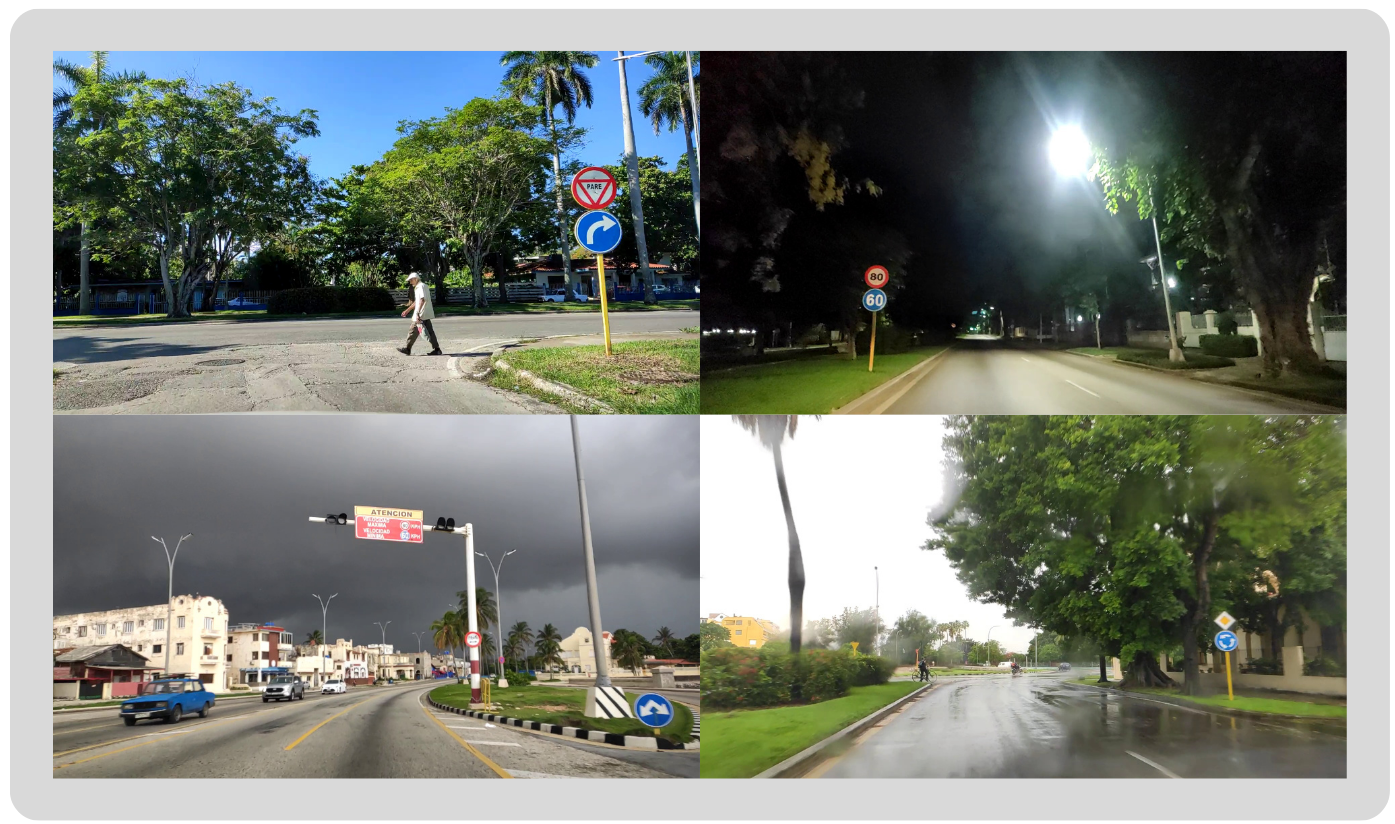
\includegraphics[width=1.0\textwidth]{resources/stages.png}
\caption{Distintos escenarios de las imágenes}
\label{fig:scenarios}
\end{figure}


Una vez obtenido el volumen de datos, comenzamos la segmentación de las señales en las imágenes. Para ello utilizamos una herramienta llamada Computer Vision Annotation Tool (CVAT) \cite{ref10}, que nos brinda una interfaz sencilla y eficiente para la anotación, además de tener un formato compatible con YOLO. Las imágenes se separaron en cuatro grupos esenciales, \textbf{Prohibición}, \textbf{Peligro}, \textbf{Obligación}, \textbf{Otras}. Del total de imágenes se obtuvieron 1011 señales, 70 de peligro, 398 de prohibición, 87 de obligación y 456 de otros tipos de señales, como se muestra en la Figura 2 \ref{fig:Grupos}.

\begin{figure}[h]
\centering
\includegraphics[width=0.9\textwidth]{resources/Grupo de señales.png}
\caption{Señales separadas por grupos}
\label{fig:Grupos}
\end{figure}

\begin{tcolorbox}
\textbf{¿Por qué CVAT?}\\
CVAT.ai es una herramienta versátil para la anotación de imágenes y videos, que sirve a la comunidad de \textit{Computer Vision} en todo el mundo. Su objetivo es ayudar a desarrolladores, empresas y organizaciones a nivel global mediante un enfoque de inteligencia artificial centrado en los datos. CVAT Cloud ofrece una plataforma robusta para la colaboración en proyectos de anotación de imágenes y videos, permitiendo a los equipos trabajar juntos de manera eficiente y efectiva, facilitando la colaboración entre diferentes miembros y departamentos.
\end{tcolorbox}

Tras tener todas las imágenes segmentadas, debemos separar los datos en los conjuntos de entrenamiento, validación y prueba. Consideramos dos formas de separar los datos:

\begin{itemize}
\item{Aleatoriamente utilizando el $20\%$ para el conjunto del prueba, y del conjunto restante, el $20\%$ para validación y el $80\%$ para entrenamiento.}
\item{Con una idea de separar proporcionalmente los datos, basado en señales que comparten cierta similitud, con el objetivo de hacer la repartición más equitativa para el modelo. Separación que además cumple los porcentajes del tipo de repartición anterior. Por lo que se realizó un conteo de las señales separándolas por dicha similitud, como se aprecia en la figura \ref{fig:sign count}}.
\end{itemize}
\begin{figure}[h]
\centering
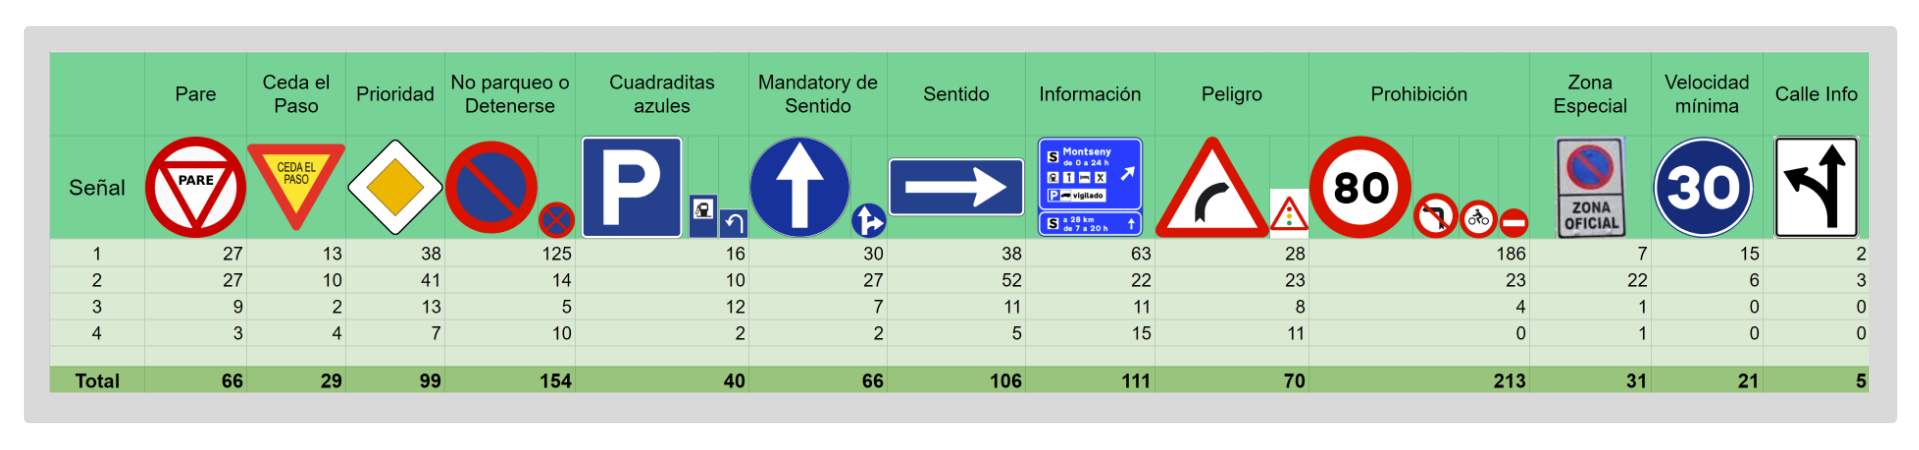
\includegraphics[width=0.9\textwidth]{resources/sign count.png}
\caption{Cantidad de señales separadas por similitud}
\label{fig:sign count}
\end{figure}
En siguiente capítulo, que trata sobre el entrenamiento de los modelos se explican las razones y usos de dichas separaciones.

\subsection{Entrenamiento y resultados del modelo}
Como ya abordamos anteriormente, partimos del modelo base \textbf{YOLOv8n} \textit{(nano)}. Este modelo es el más ligero de la familia YOLOv8 y consta de 24 capas y 3.2 millones de parámetros. YOLOv8n ha demostrado un comportamiento al nivel del estado del arte en conjuntos de datos populares como COCO y VOC. 

YOLO es una excelente opción para Transfer Learning debido a su arquitectura pre-entrenada que sobresale en la extracción de características. Esto permite que, al aplicarse \textit{Transfer Learning}, el modelo ya cuente con una sólida base de características previamente aprendidas, lo que acelera y mejora el proceso de entrenamiento en nuevos dominios o con datos específicos. 

En la primera etapa de la solución entrenamos el modelo en el conjunto de datos GTSRB, con el objetivo de que aprenda a reconocer algunas señales. Para ello decidimos hacer \textit{Transfer Learning} definiendo las primeras 5 épocas como \textit{épocas de calentamiento} y manteniendo invariables los parámetros de las 10 primeras capas, a las que se le conoce como el \textit{backbone} de YOLOv8n, las cuales se encargan de la extracción de características. Este modelo basado en GTSRB se guarda en el archivo $general\_best.pt$.

Una vez entrenado nuestro modelo inicial, evaluamos sus resultados con ambos conjuntos de datos (CTSRD y GTSRB)(figura \ref{fig:results in general}).

\begin{figure}[h]
\begin{subfigure}[b]{0.5\textwidth}
\centering
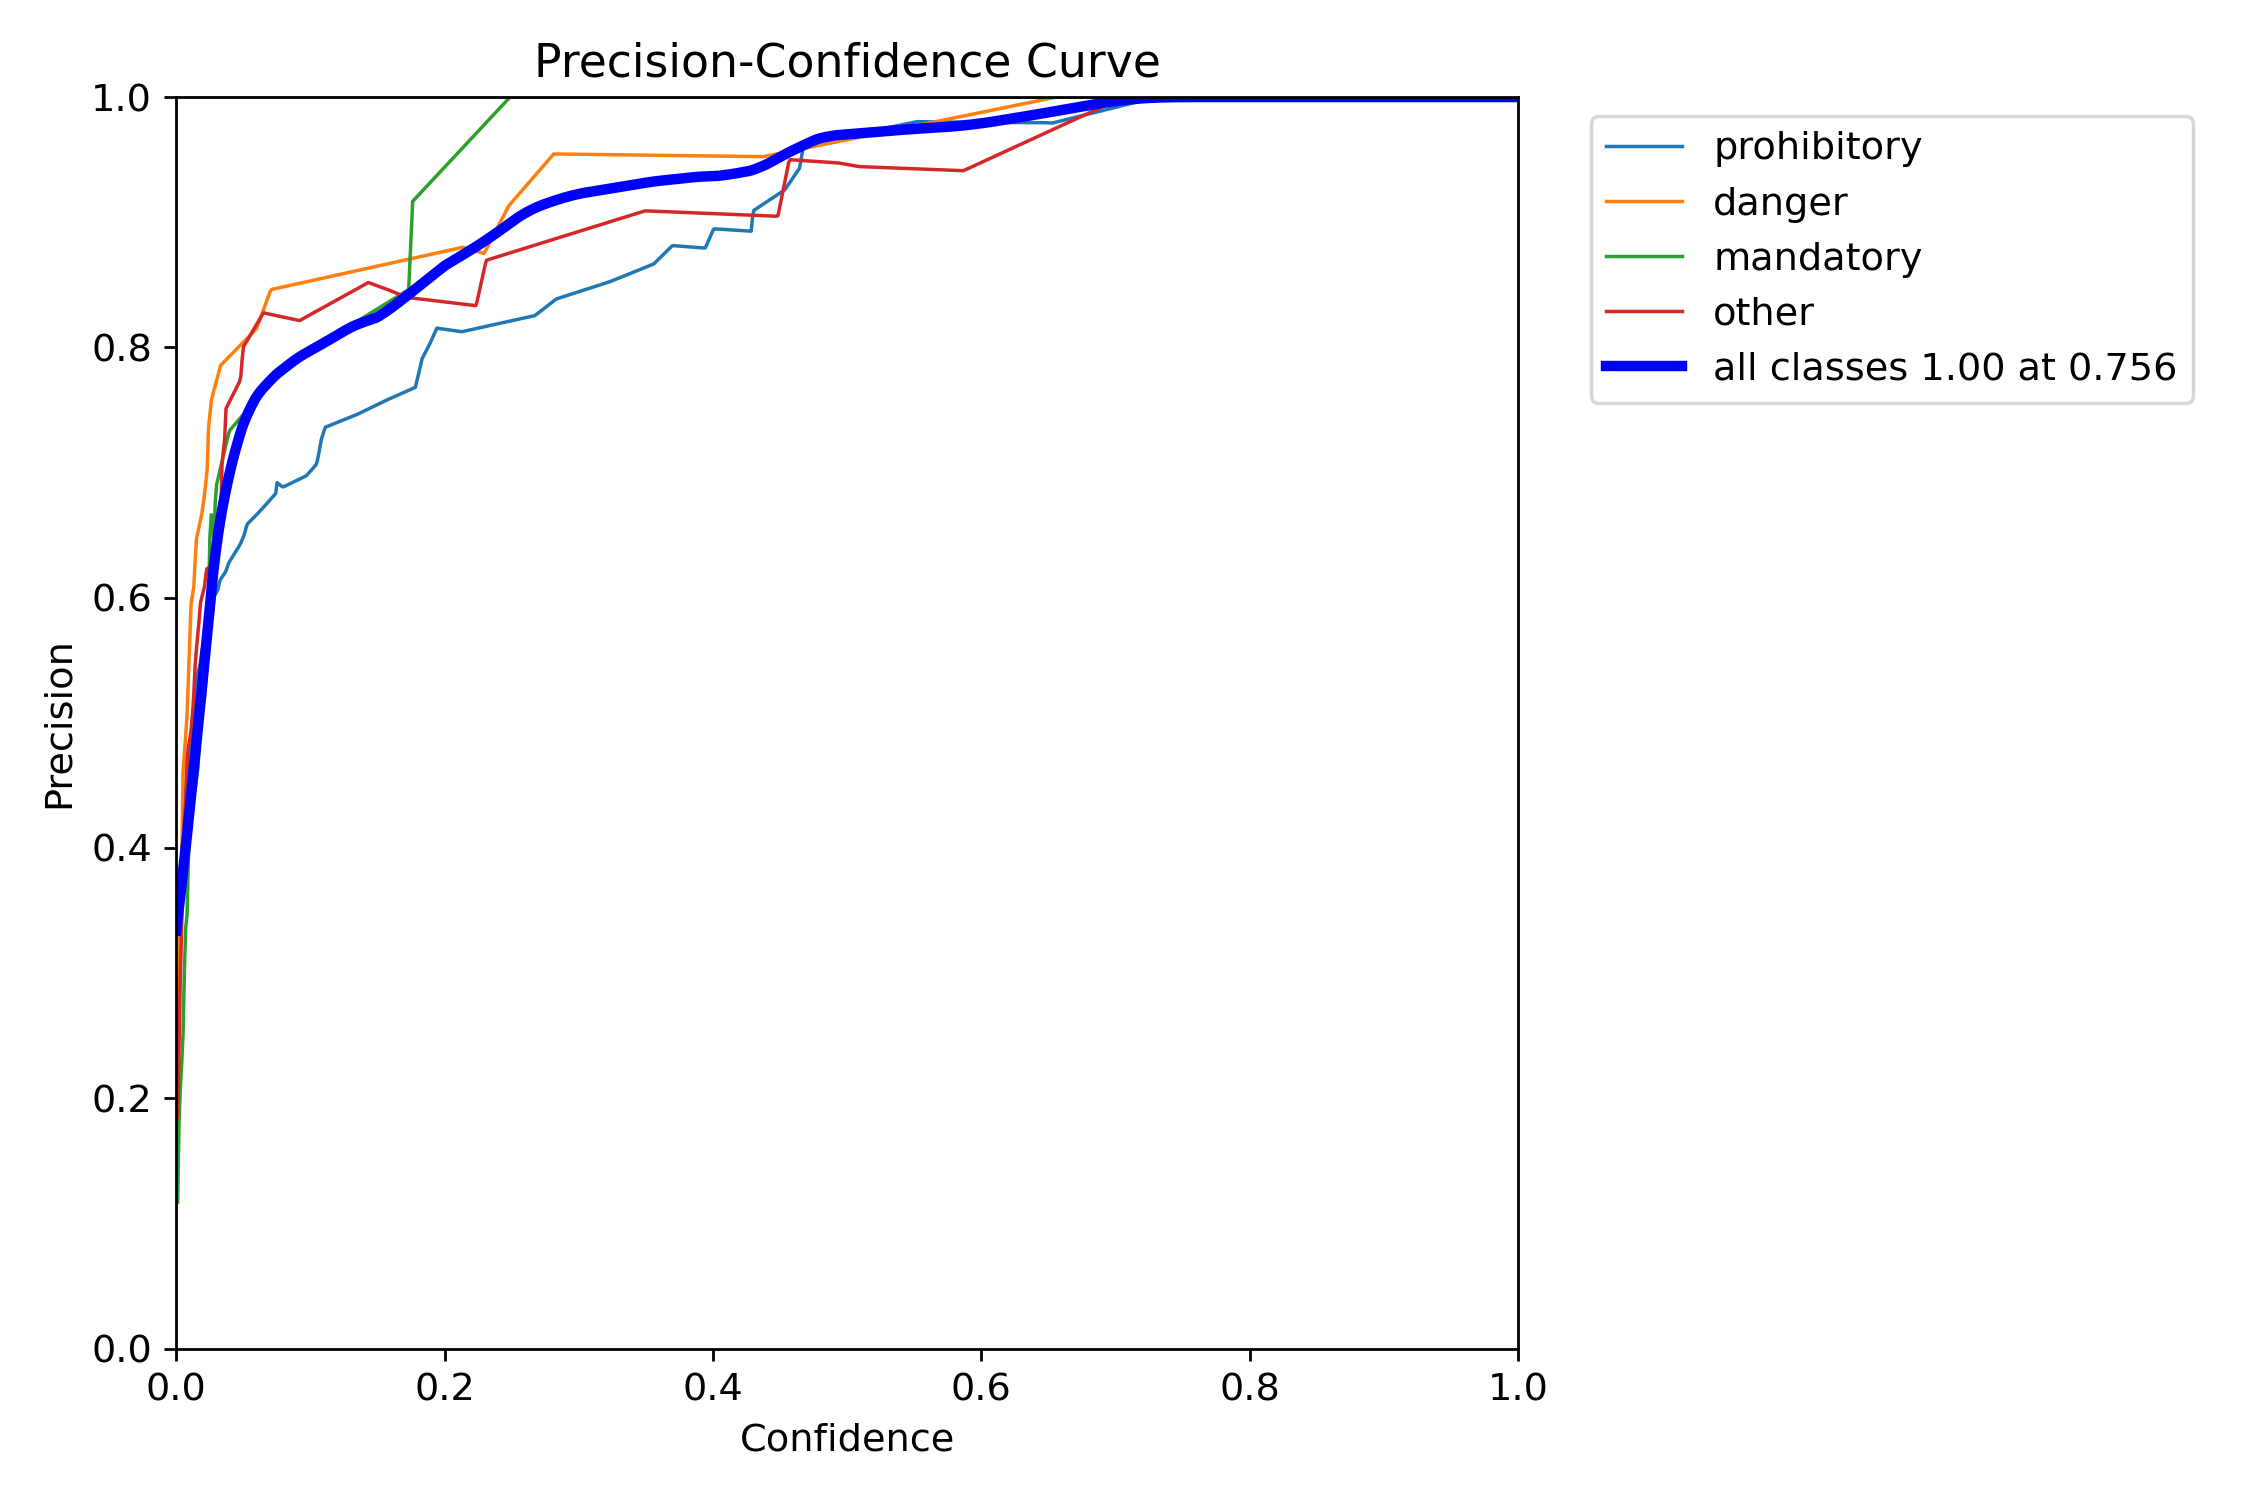
\includegraphics[width=0.9\textwidth]{resources/general in general P curve.png}
\caption{}
\end{subfigure}
\begin{subfigure}[b]{0.5\textwidth}
\centering
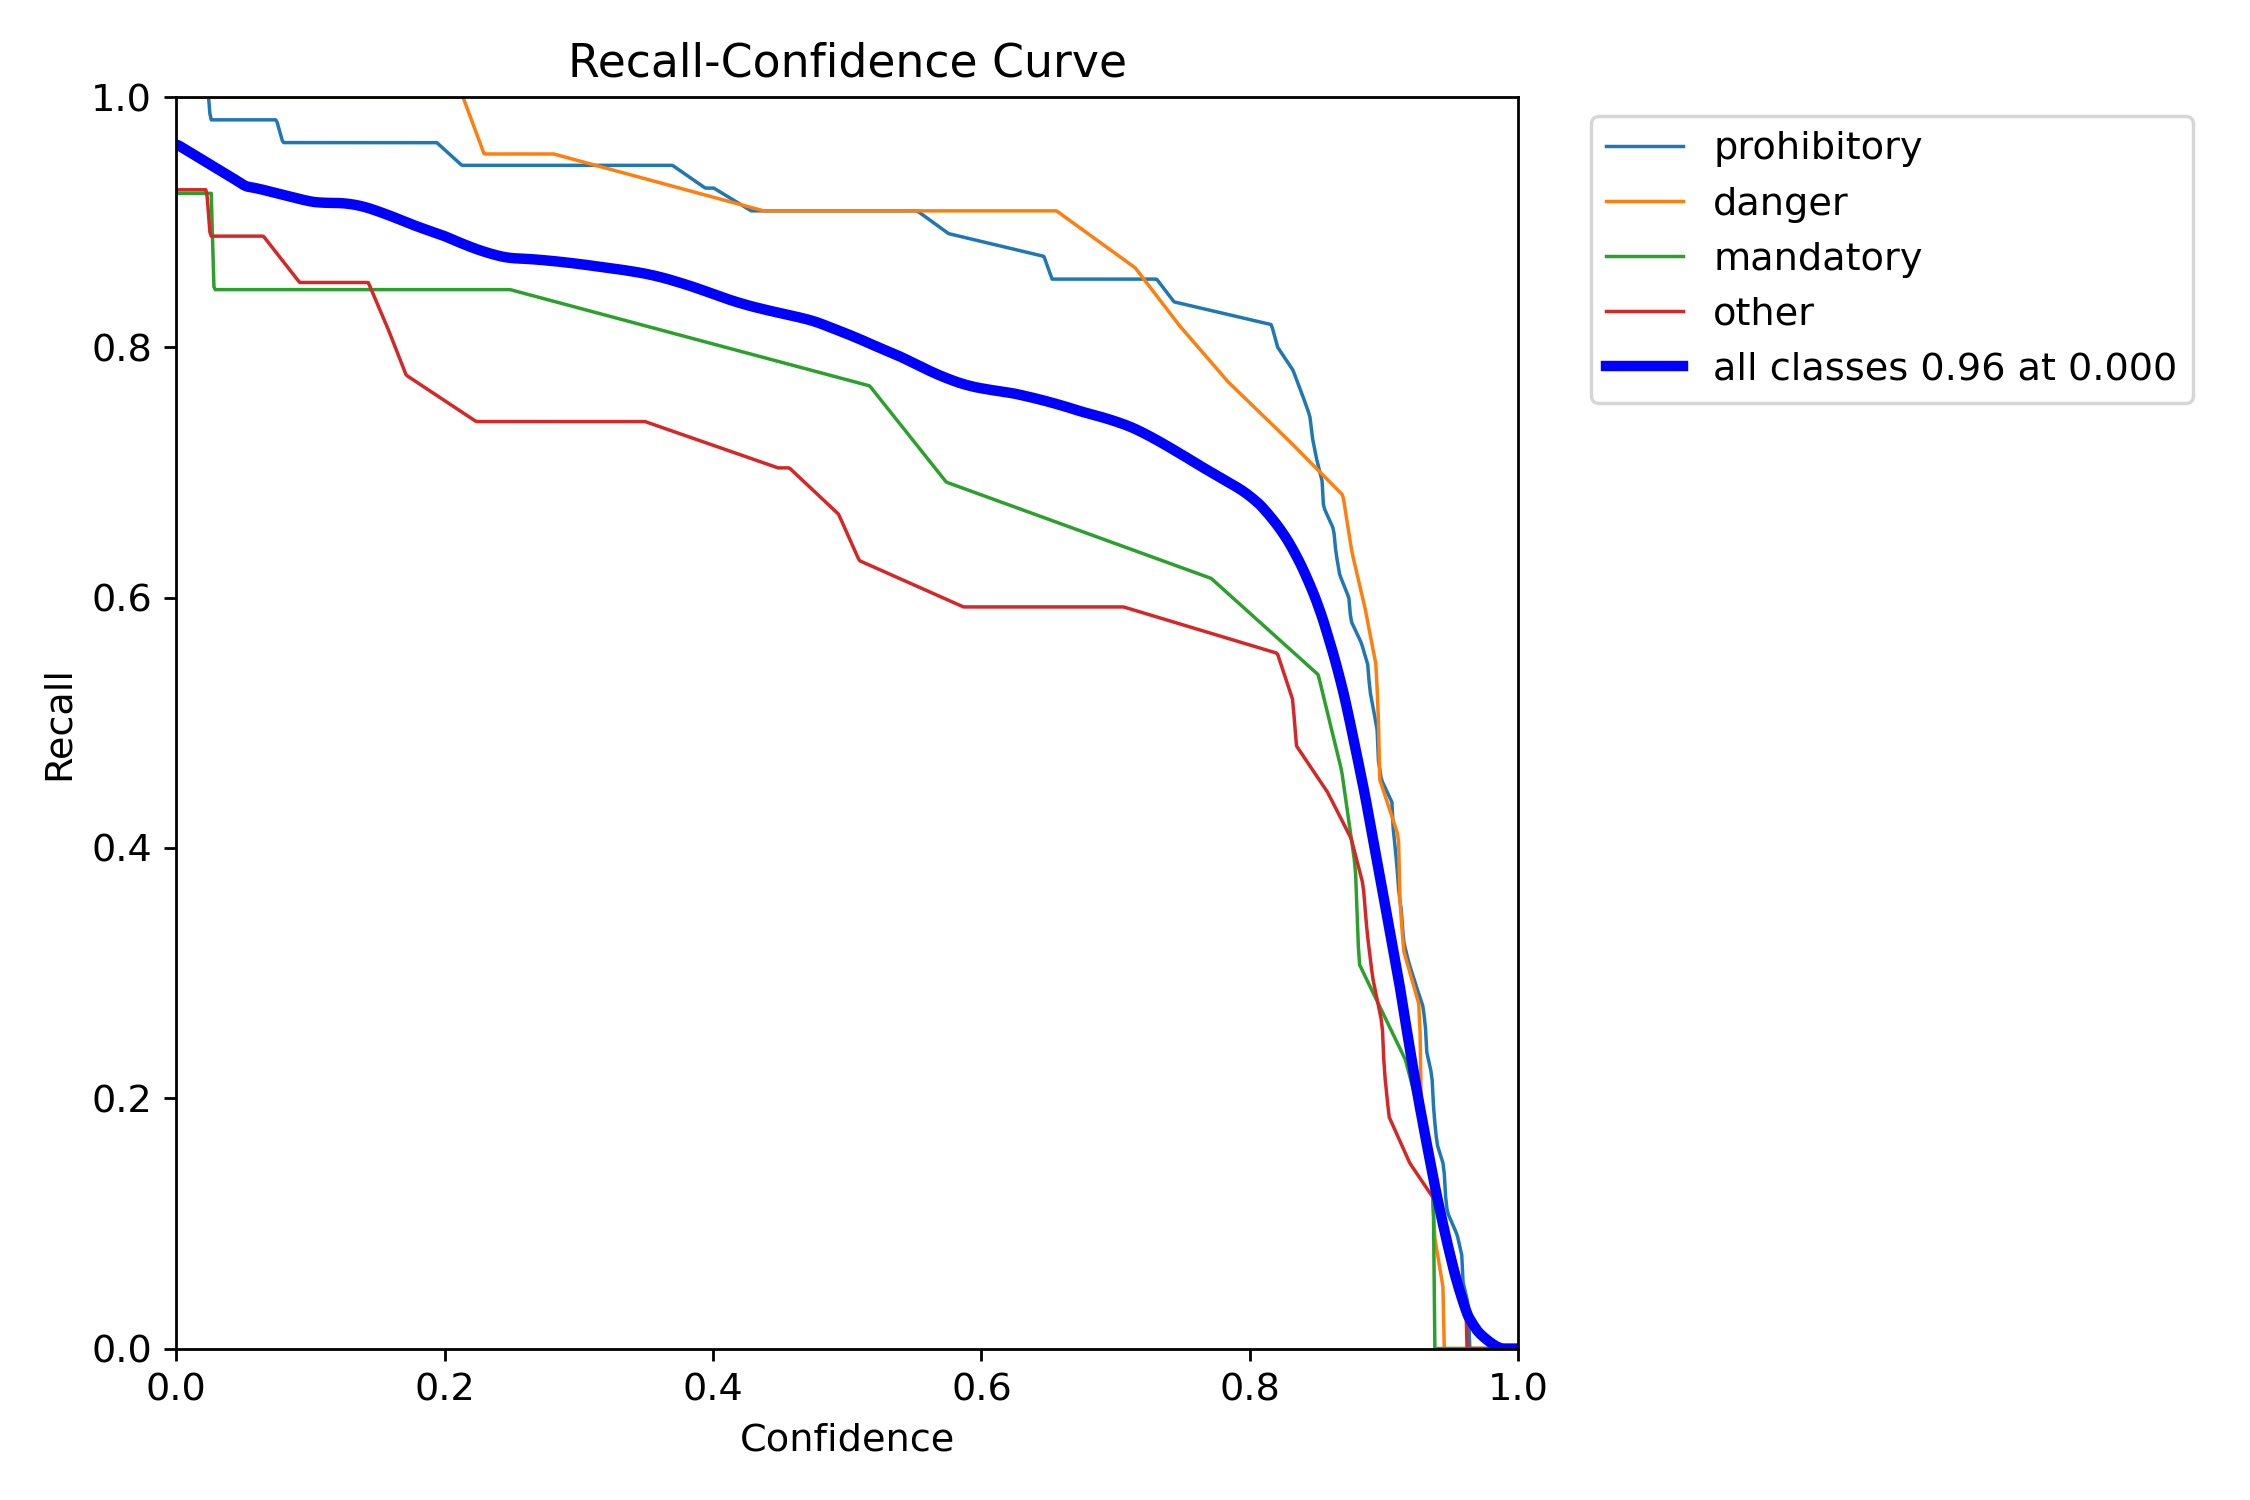
\includegraphics[width=0.9\textwidth]{resources/general in general R curve.png}
\caption{}
\end{subfigure}
\begin{subfigure}[b]{0.5\textwidth}
\centering
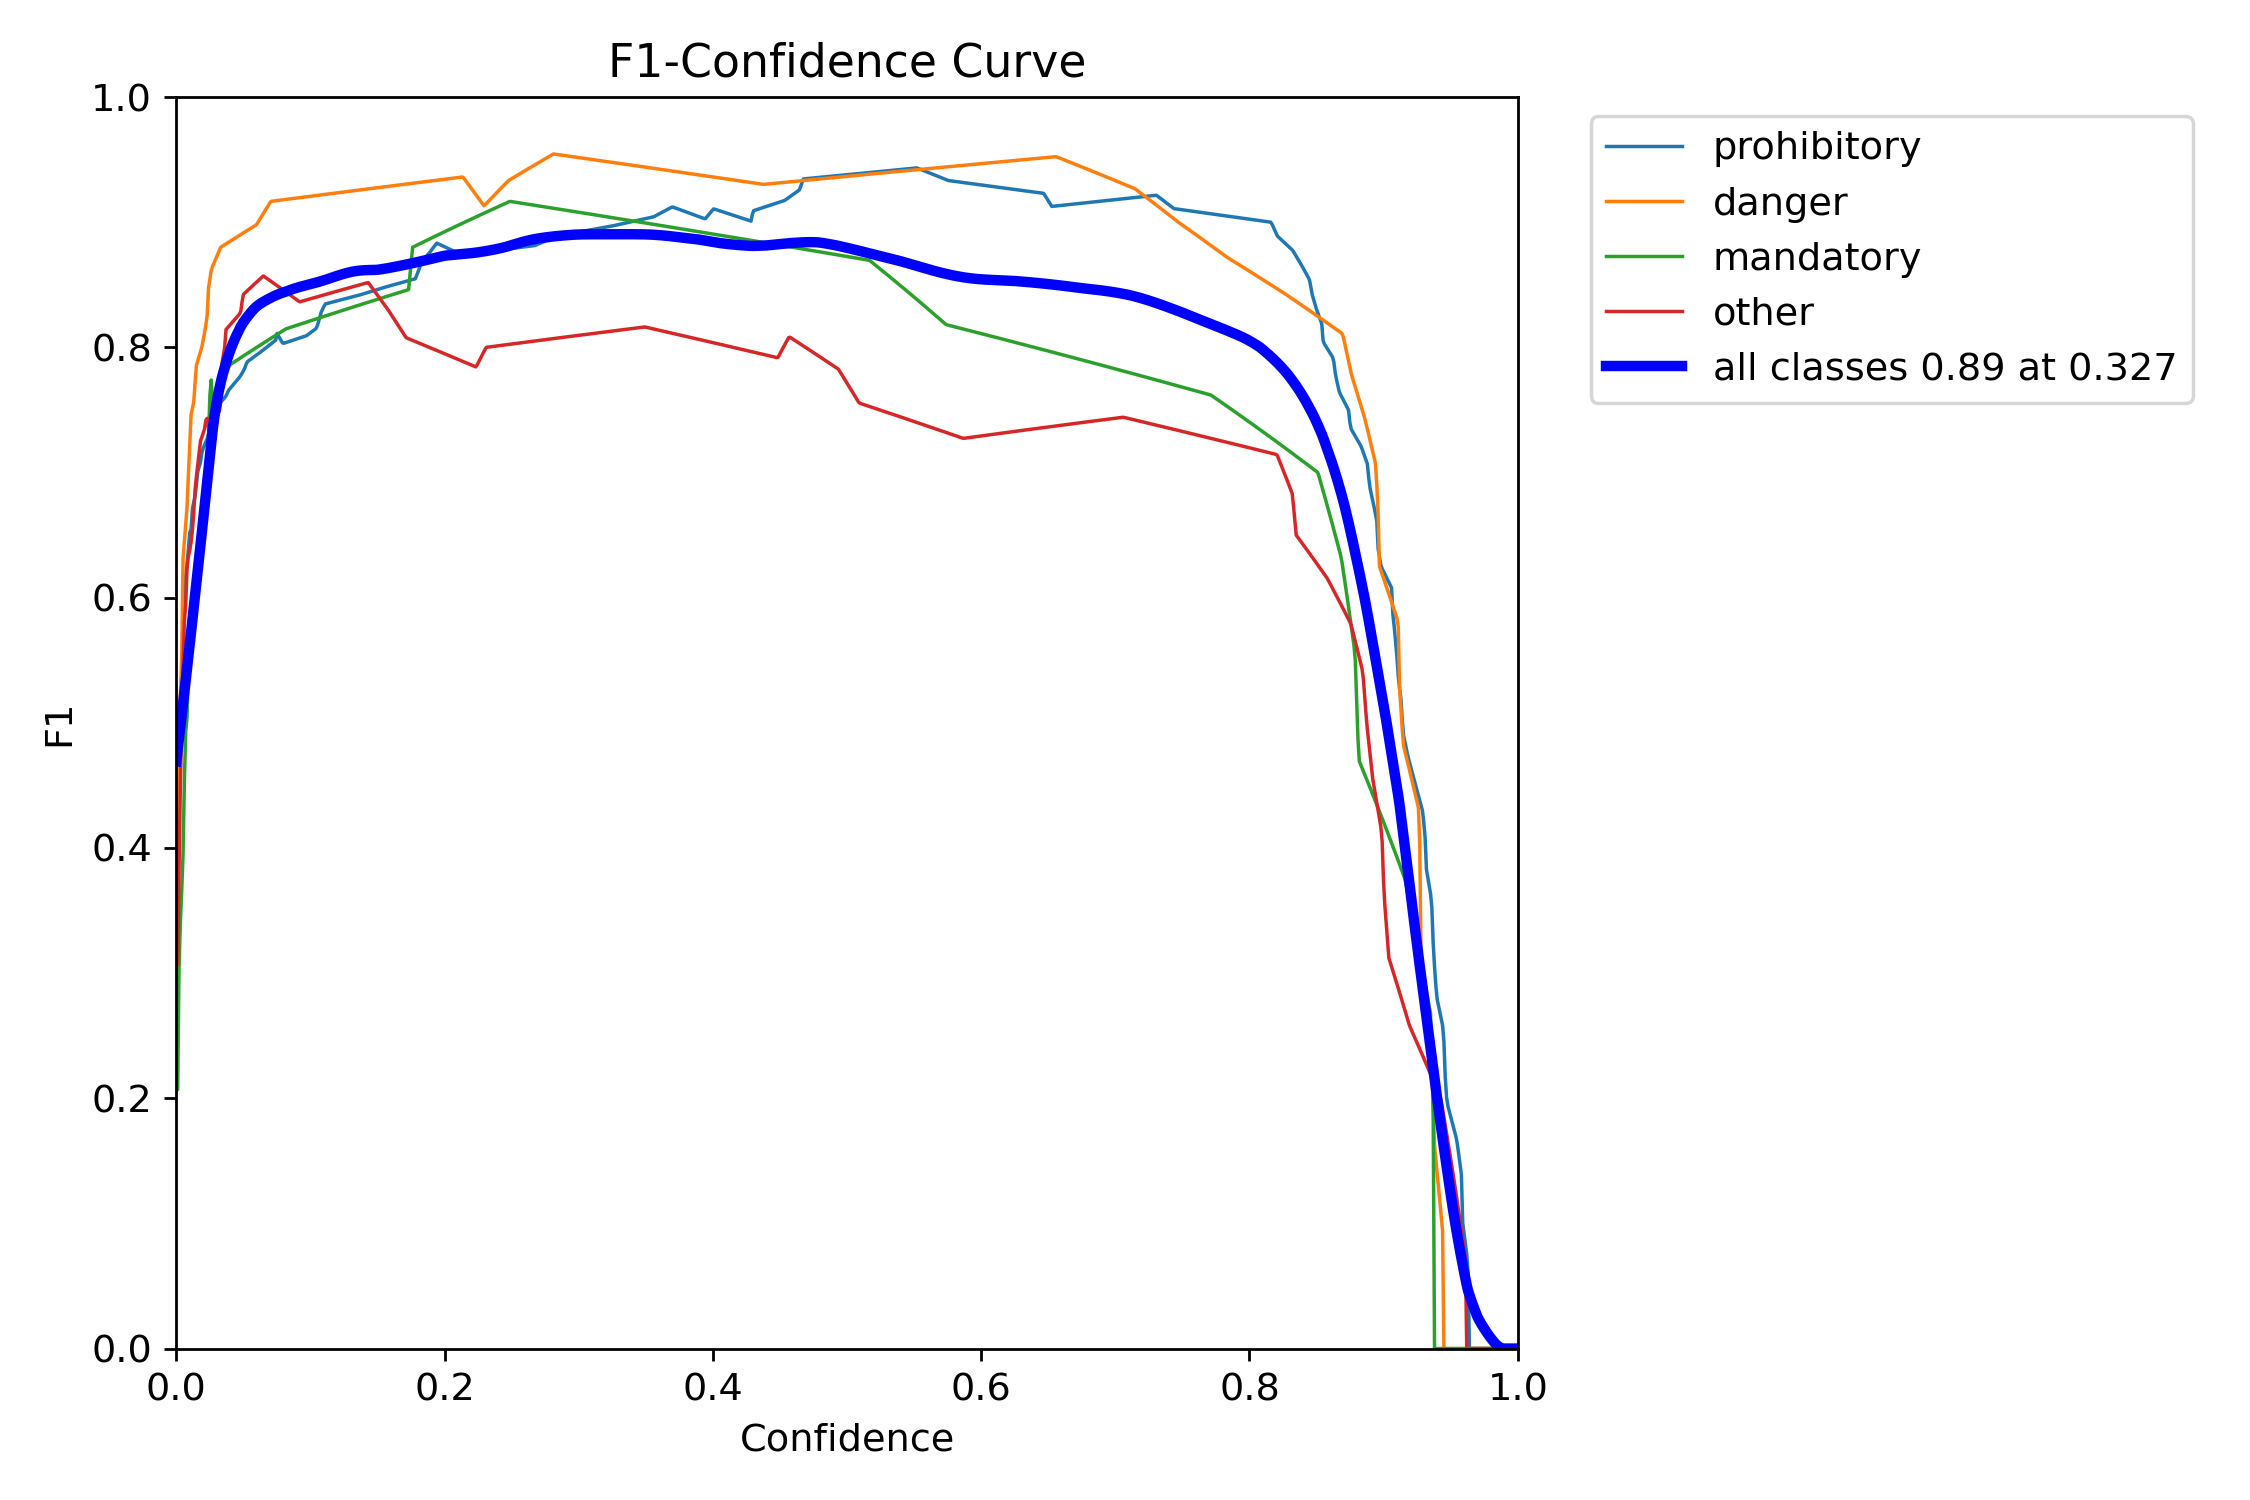
\includegraphics[width=0.9\textwidth]{resources/general in general F1 curve.png}
\caption{}
\end{subfigure}
\begin{subfigure}[b]{0.5\textwidth}
\centering
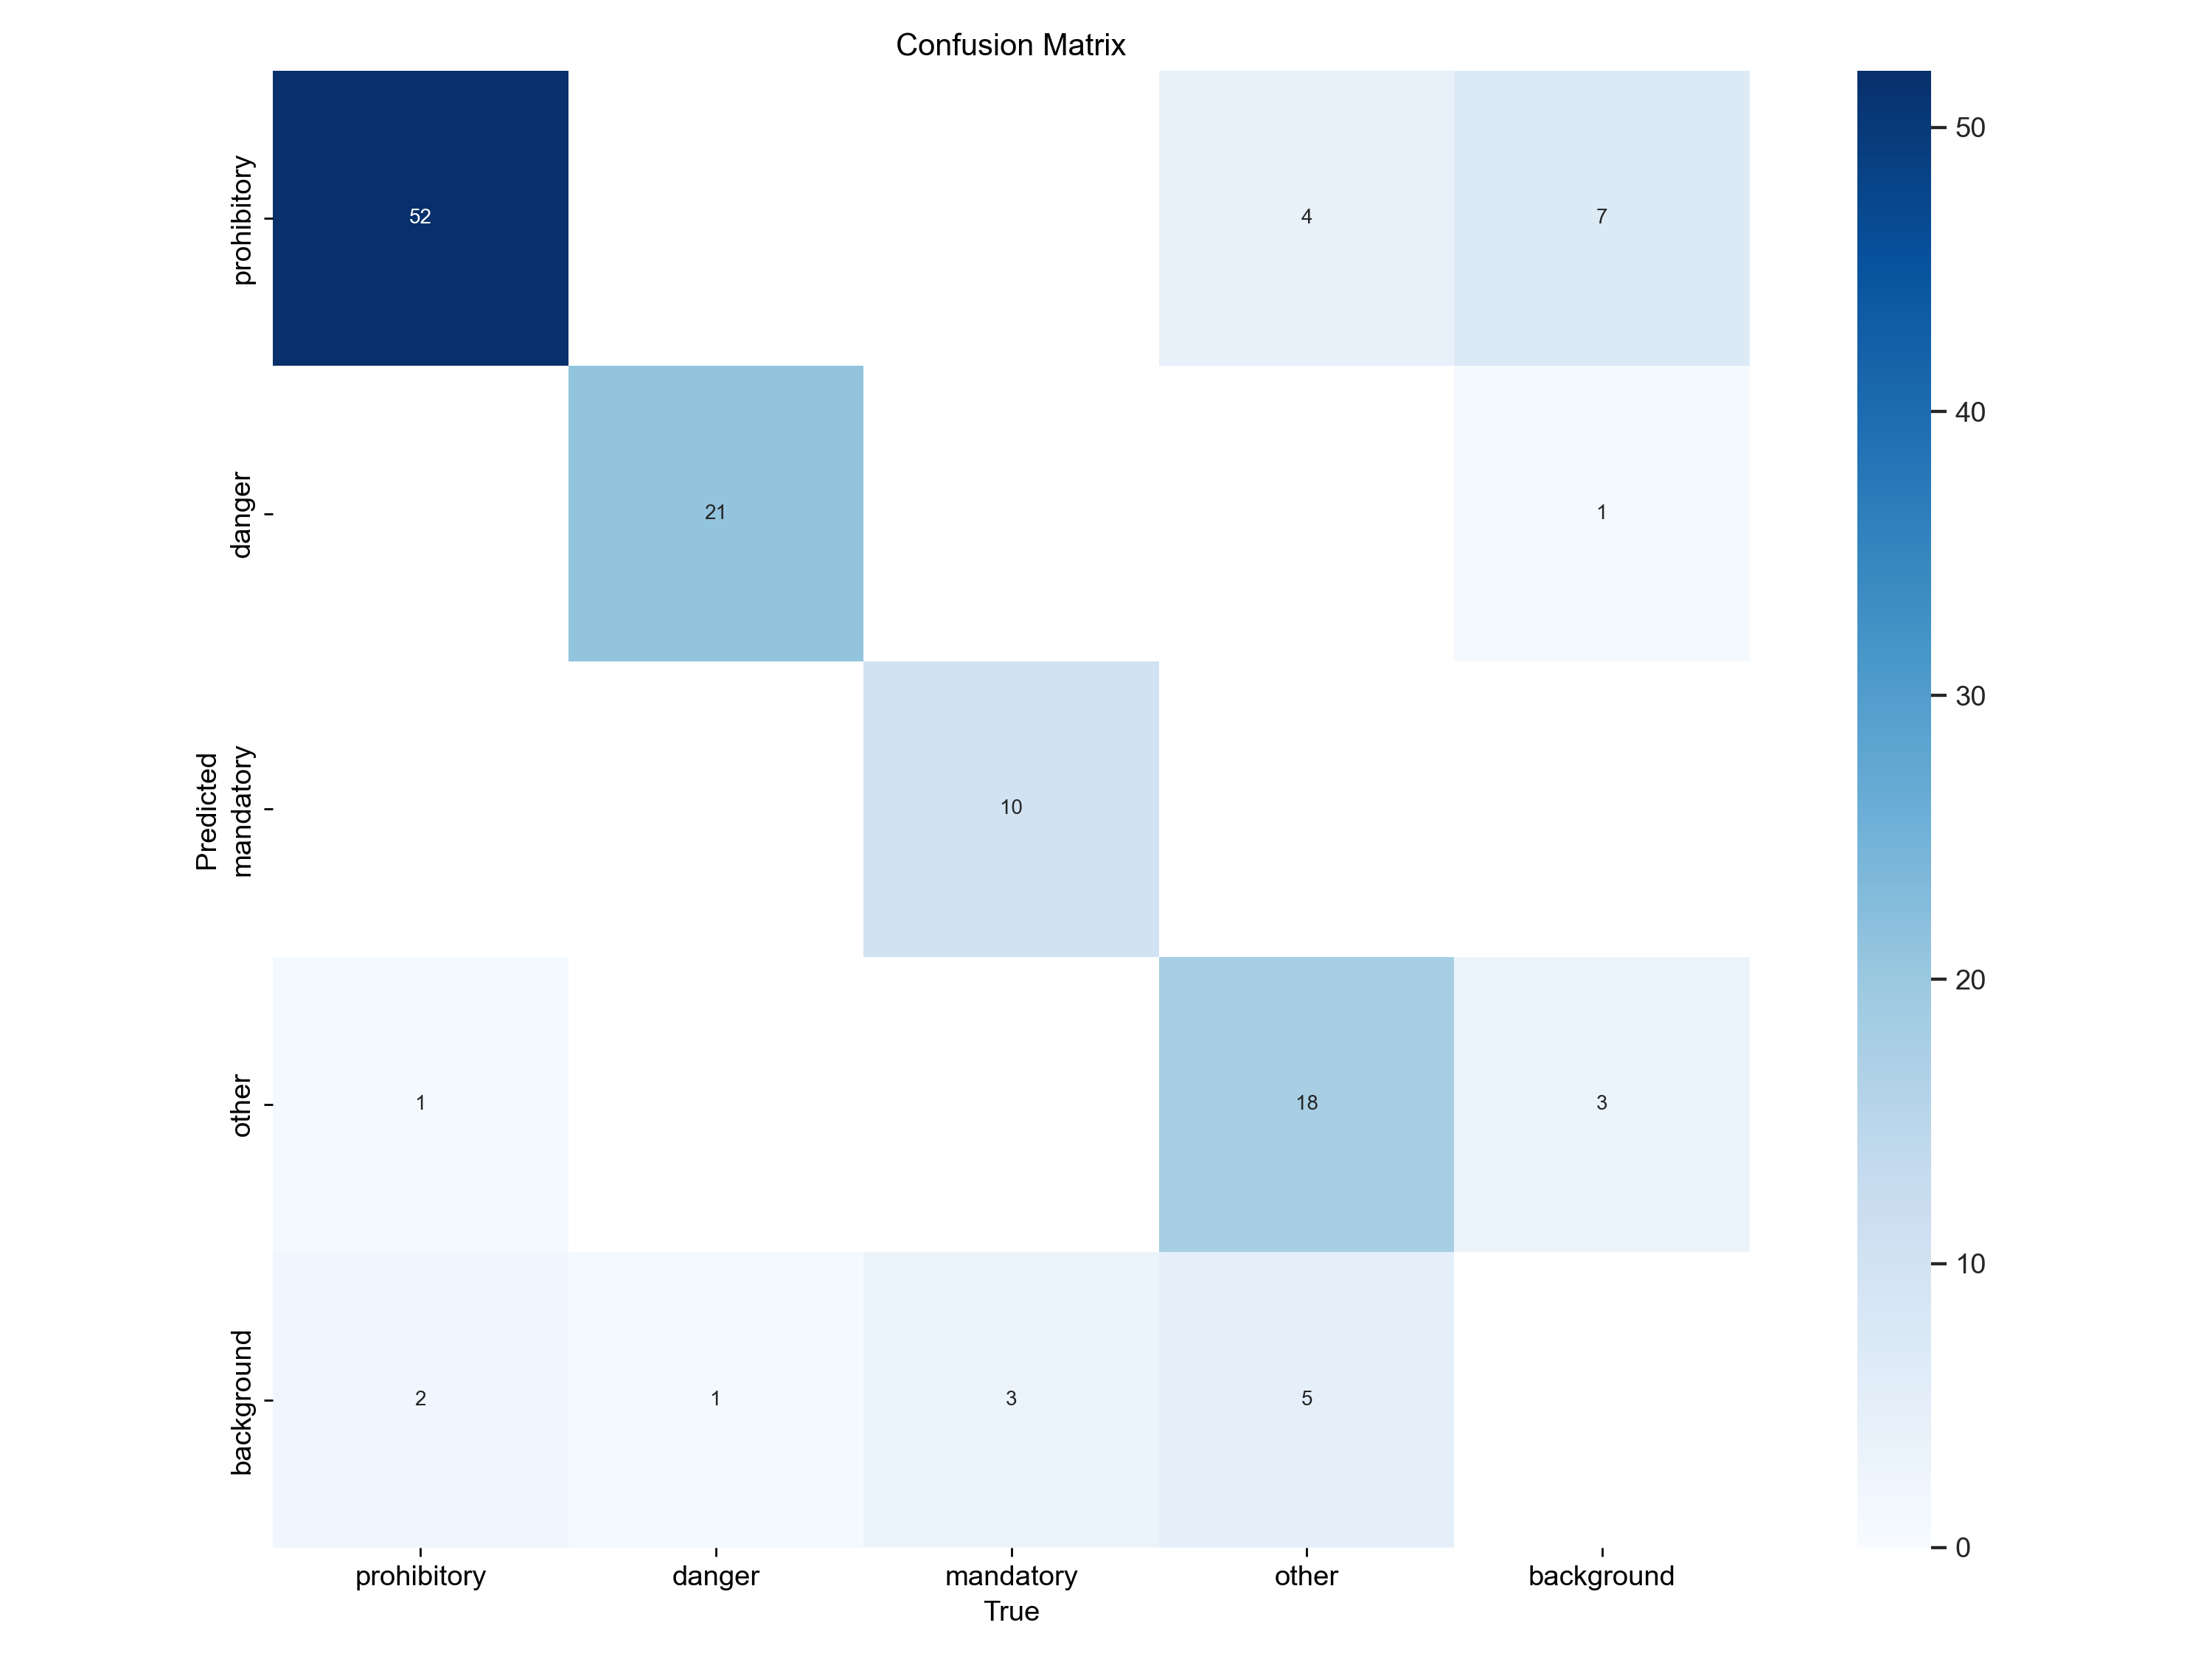
\includegraphics[width=0.9\textwidth]{resources/general in general confusion matrix.png}
\caption{}
\end{subfigure}
\caption{Métricas en el conjunto GTSRB. a) Curva de precisión b) Curva de recobrado c) F1 d) Matriz de confusión}
\label{fig:results in general}
\end{figure}

Como se puede apreciar en los gráficos anteriores, podemos concluir que el modelo posee un buen desempeño en las imágenes de prueba del conjunto de imágenes de la misma naturaleza del conjunto donde fue entrenado. Se puede observar como para niveles no muy exigentes de confianza, el modelo obtiene una excelente precisión, además en la gráfica de recobrado obtenemos buenos valores para poca confianza y la pendiente de descenso no es tan pronunciada inicialmente. Además, si analizamos la matriz de confusión, se puede observar que el mayor problema que presenta, es que reconoce señales donde no debe haberlas y reconoce señales donde no las hay. Si analizamos la gráfica de la métrica F1 se puede apreciar que para los valores centrales de confianza tanto la precisión como el recobrado son bastante altos y estables, solo obteniendo un descenso brusco para valores muy altos (por encima de 0.8) de confianza.

De forma general observamos buenas métricas en la evaluación anterior, sin embargo ¿Qué pasa si evaluamos en los datos de CTSRD?

\begin{figure}[h]
\begin{subfigure}[b]{0.5\textwidth}
\centering
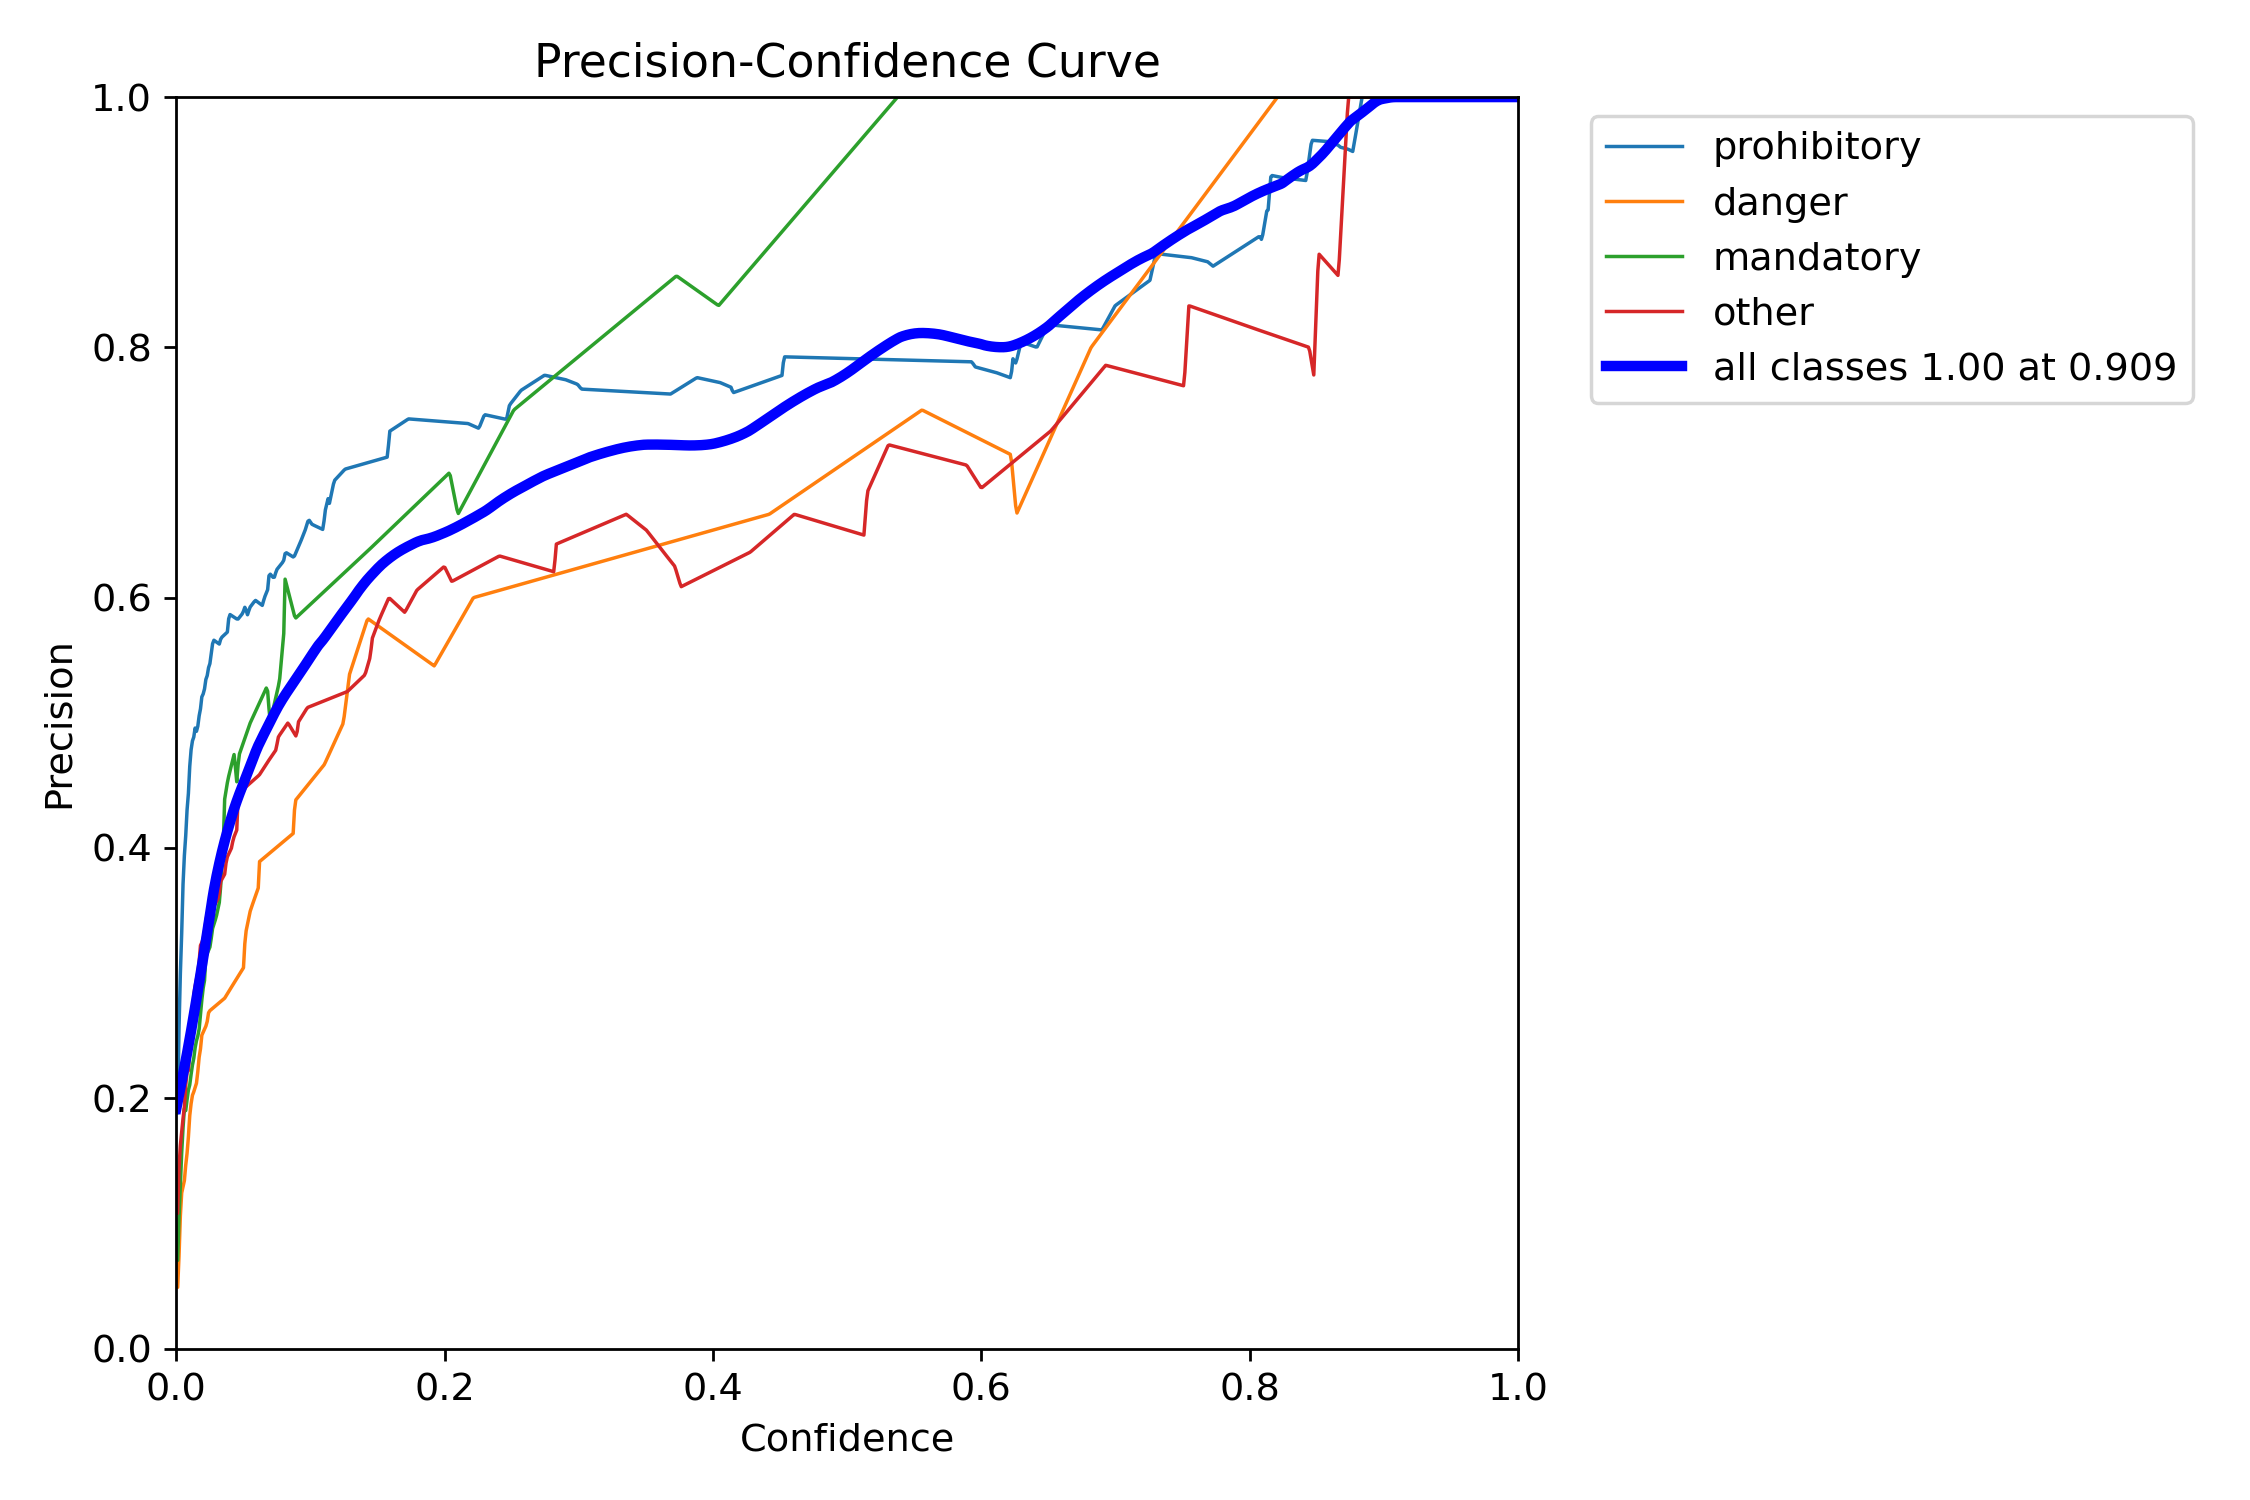
\includegraphics[width=0.9\textwidth]{resources/cuban in general P curve.png}
\caption{}
\end{subfigure}
\begin{subfigure}[b]{0.5\textwidth}
\centering
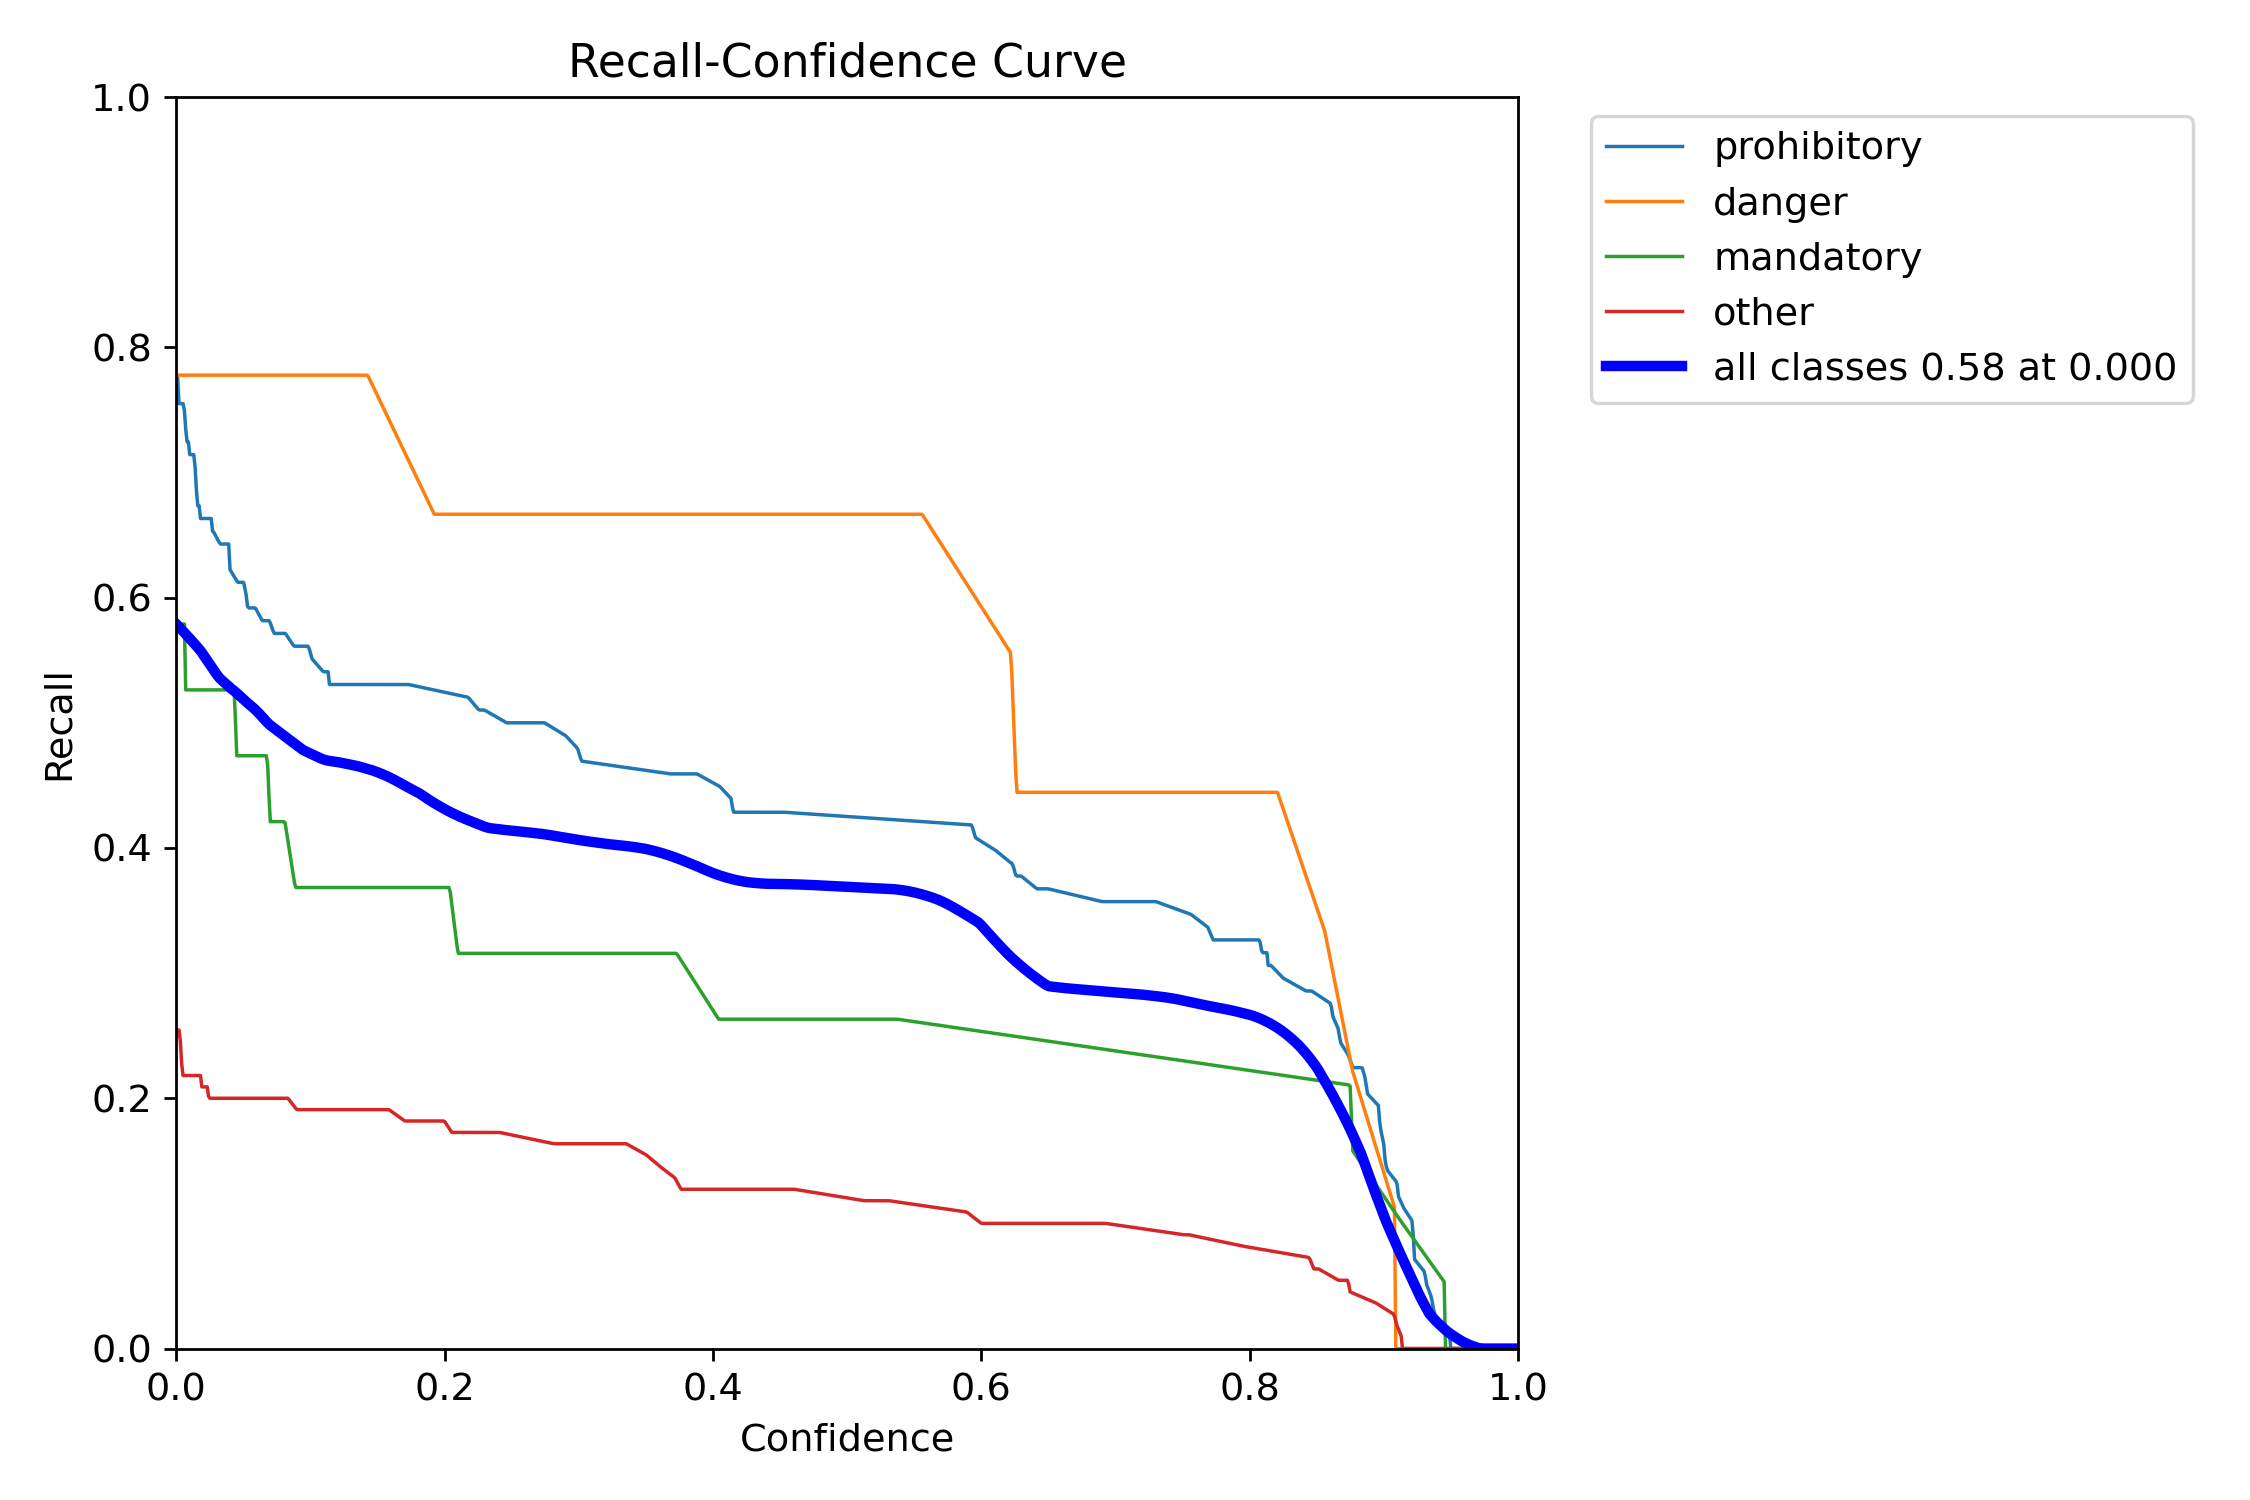
\includegraphics[width=0.9\textwidth]{resources/cuban in general R curve.png}
\caption{}
\end{subfigure}
\begin{subfigure}[b]{0.5\textwidth}
\centering
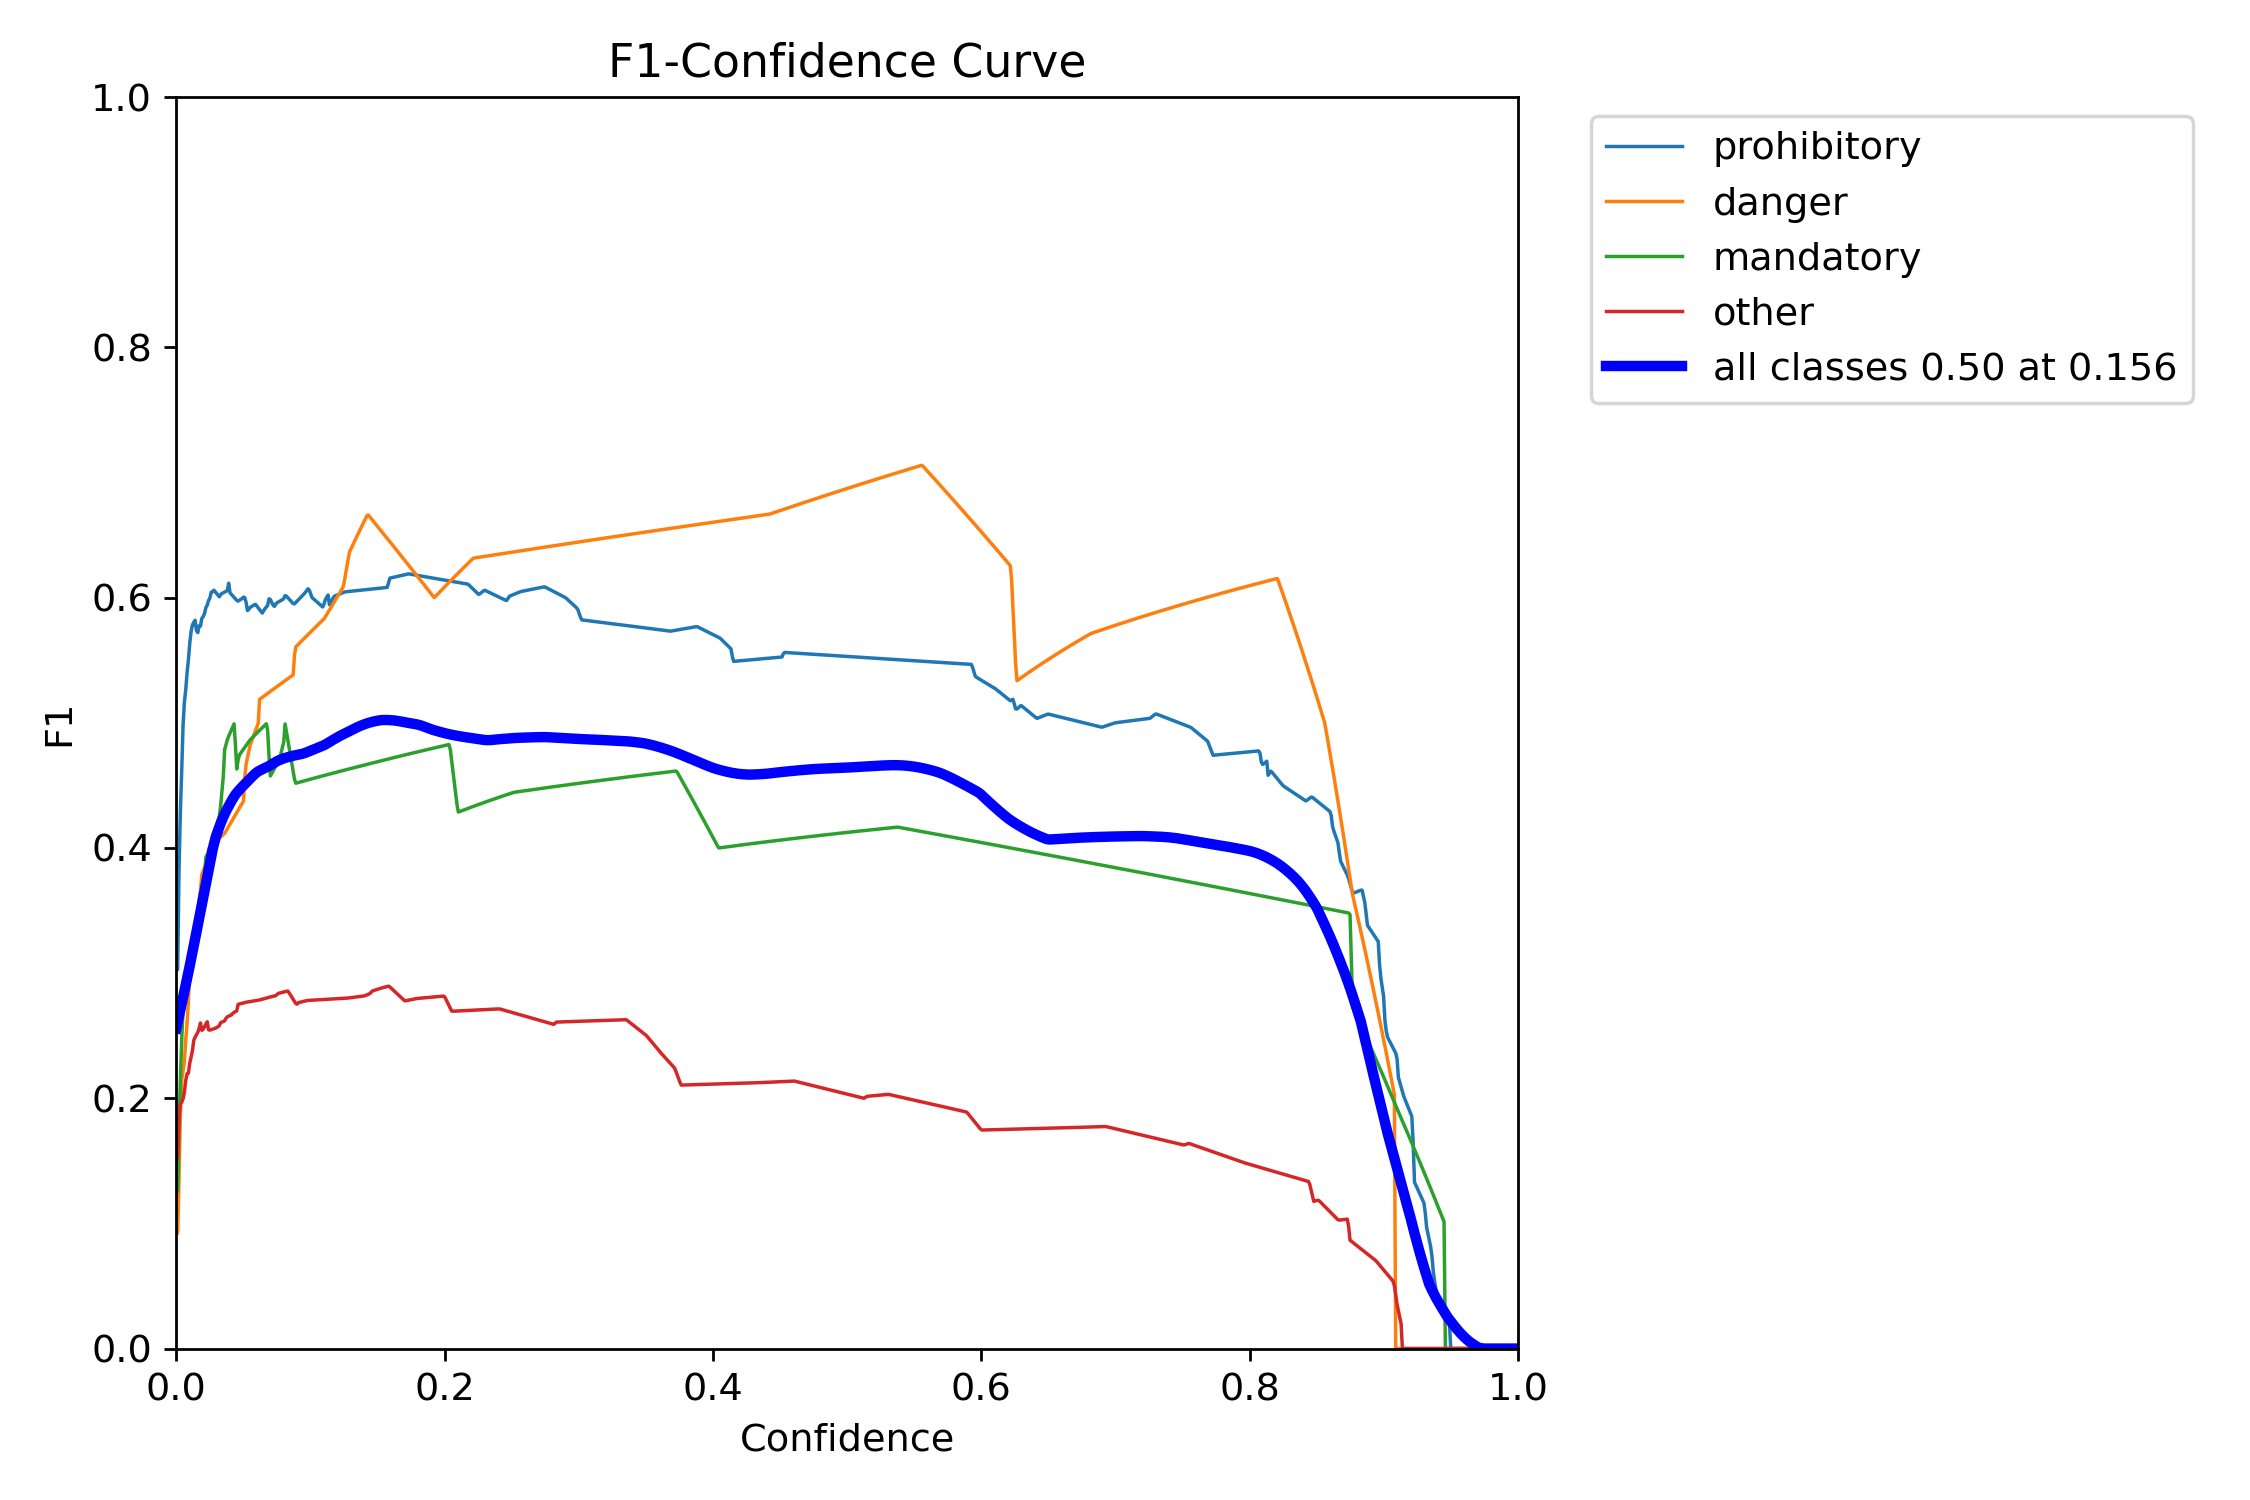
\includegraphics[width=0.9\textwidth]{resources/cuban in general F1 curve.png}
\caption{}
\end{subfigure}
\begin{subfigure}[b]{0.5\textwidth}
\centering
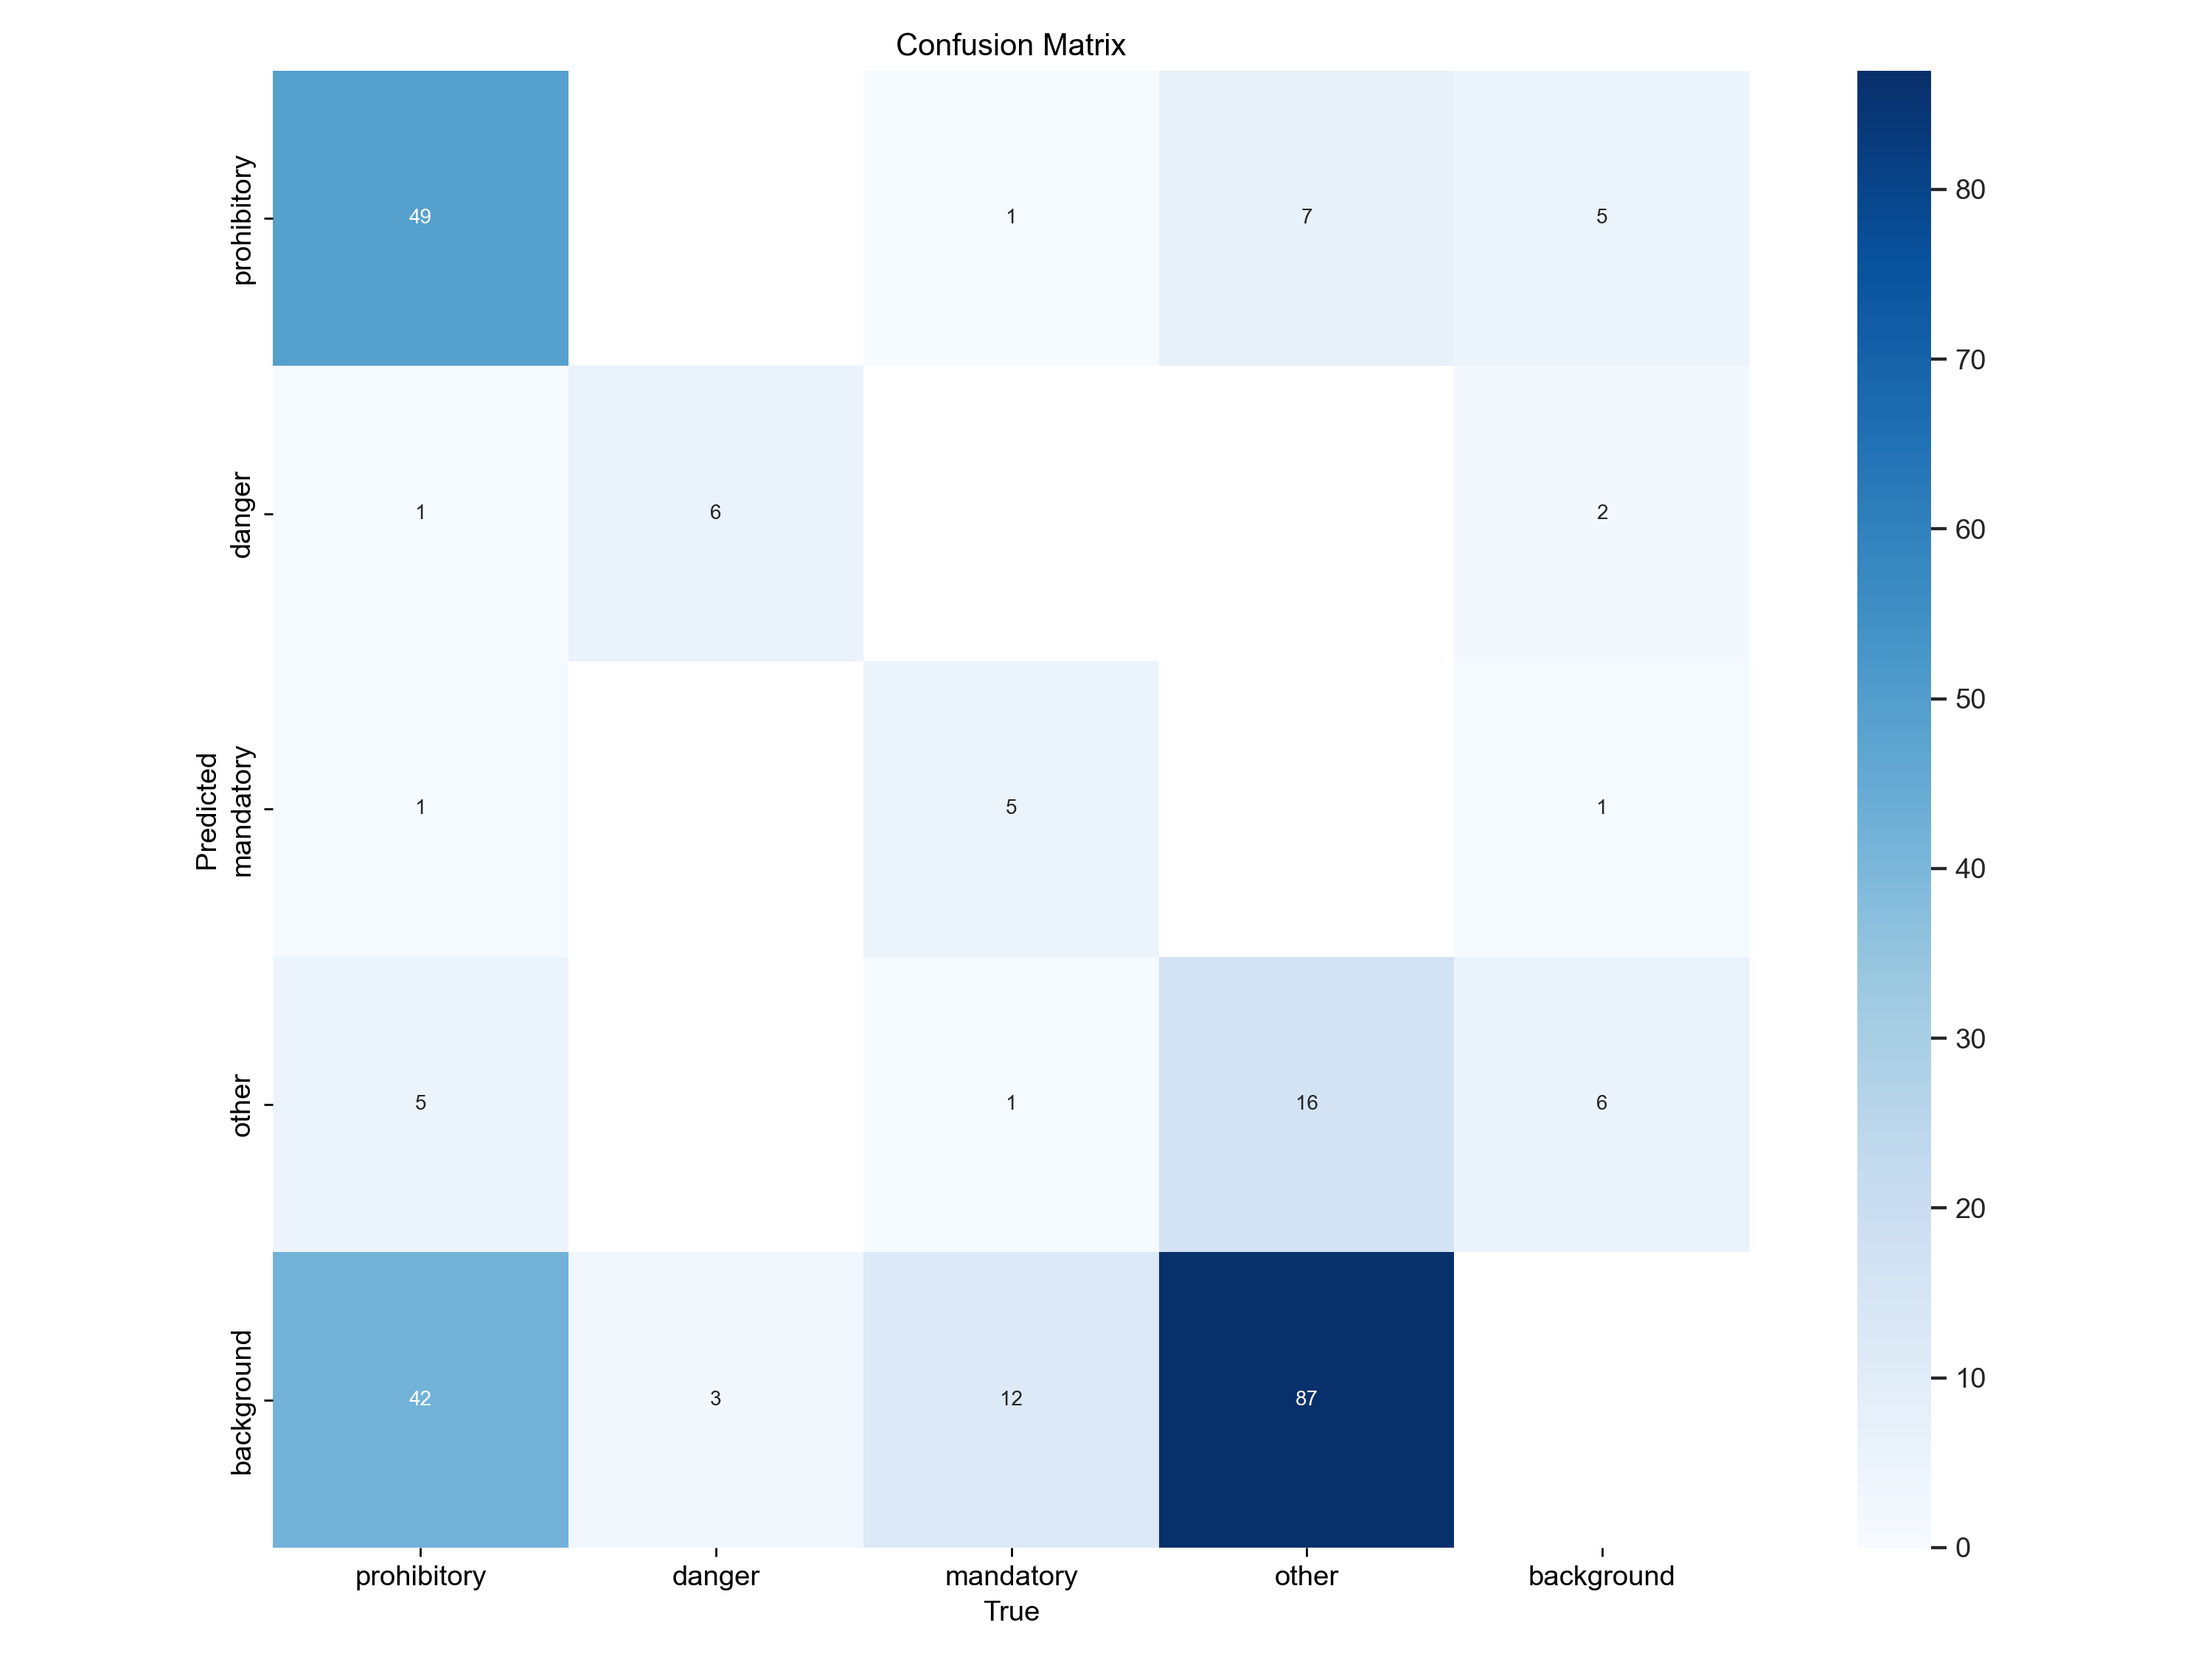
\includegraphics[width=0.9\textwidth]{resources/cuban in general confusion matrix.png}
\caption{}
\end{subfigure}
\caption{Métricas en el conjunto CTSRD. a) Curva de precisión b) Curva de recobrado c) F1 d) Matriz de confusión}
\label{fig:results in cuban general}
\end{figure}

Al observar los resultados (Figura \ref{fig:results in cuban general}) en este conjunto de datos, es evidente el mal desempeño del modelo. Una de las razones de este mal desempeño es la heterogeneidad de las características que describen a las señales de ambos conjuntos (Figura 6), por no mencionar los metadatos de las imágenes. Lo anterior expuesto nos lleva a la necesidad de hacer un nuevo entrenamiento sobre el modelo $general\_best.pt$ con los datos del conjunto CTSRD.

\begin{figure}[h]
\centering
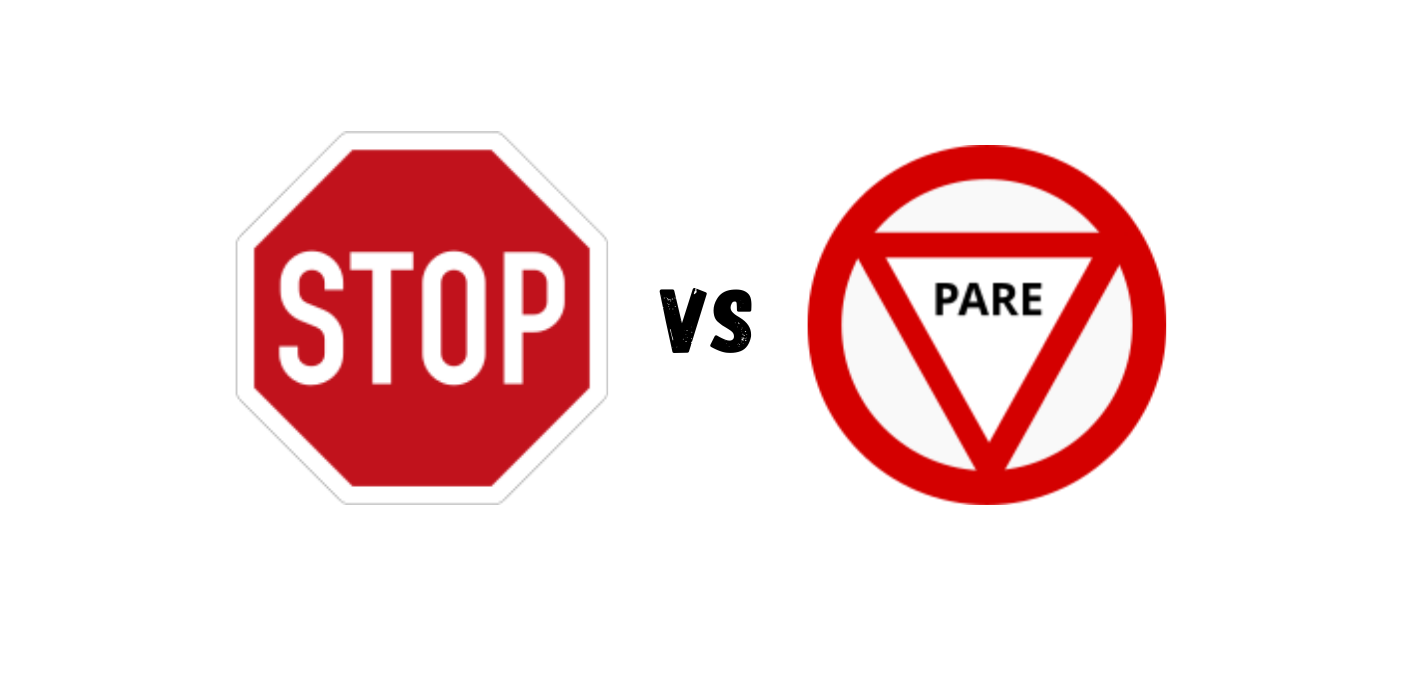
\includegraphics[width=0.4\textwidth]{resources/vs.png}
\caption{Ejemplos de pare en ambos conjuntos}
\label{fig:vs}
\end{figure}

Para enfrentar esta problemática propusimos dos soluciones de entrenamiento diferenciada por la forma de repartir los datos, explicadas en la sección anterior. La división aleatoria fue la primera aproximación ingenua (modelo $cuban\_rand.pt$), por otra parte, la segunda separación llega como una alternativa más equilibrada para el modelo, en aras de dotar de heterogeneidad en los conjuntos de entrenamiento, validación y prueba (modelo $cuban\_sim.pt$). Comparemos los resultados de ambos modelos.

\begin{figure}[h]
\begin{subfigure}[b]{0.5\textwidth}
\centering
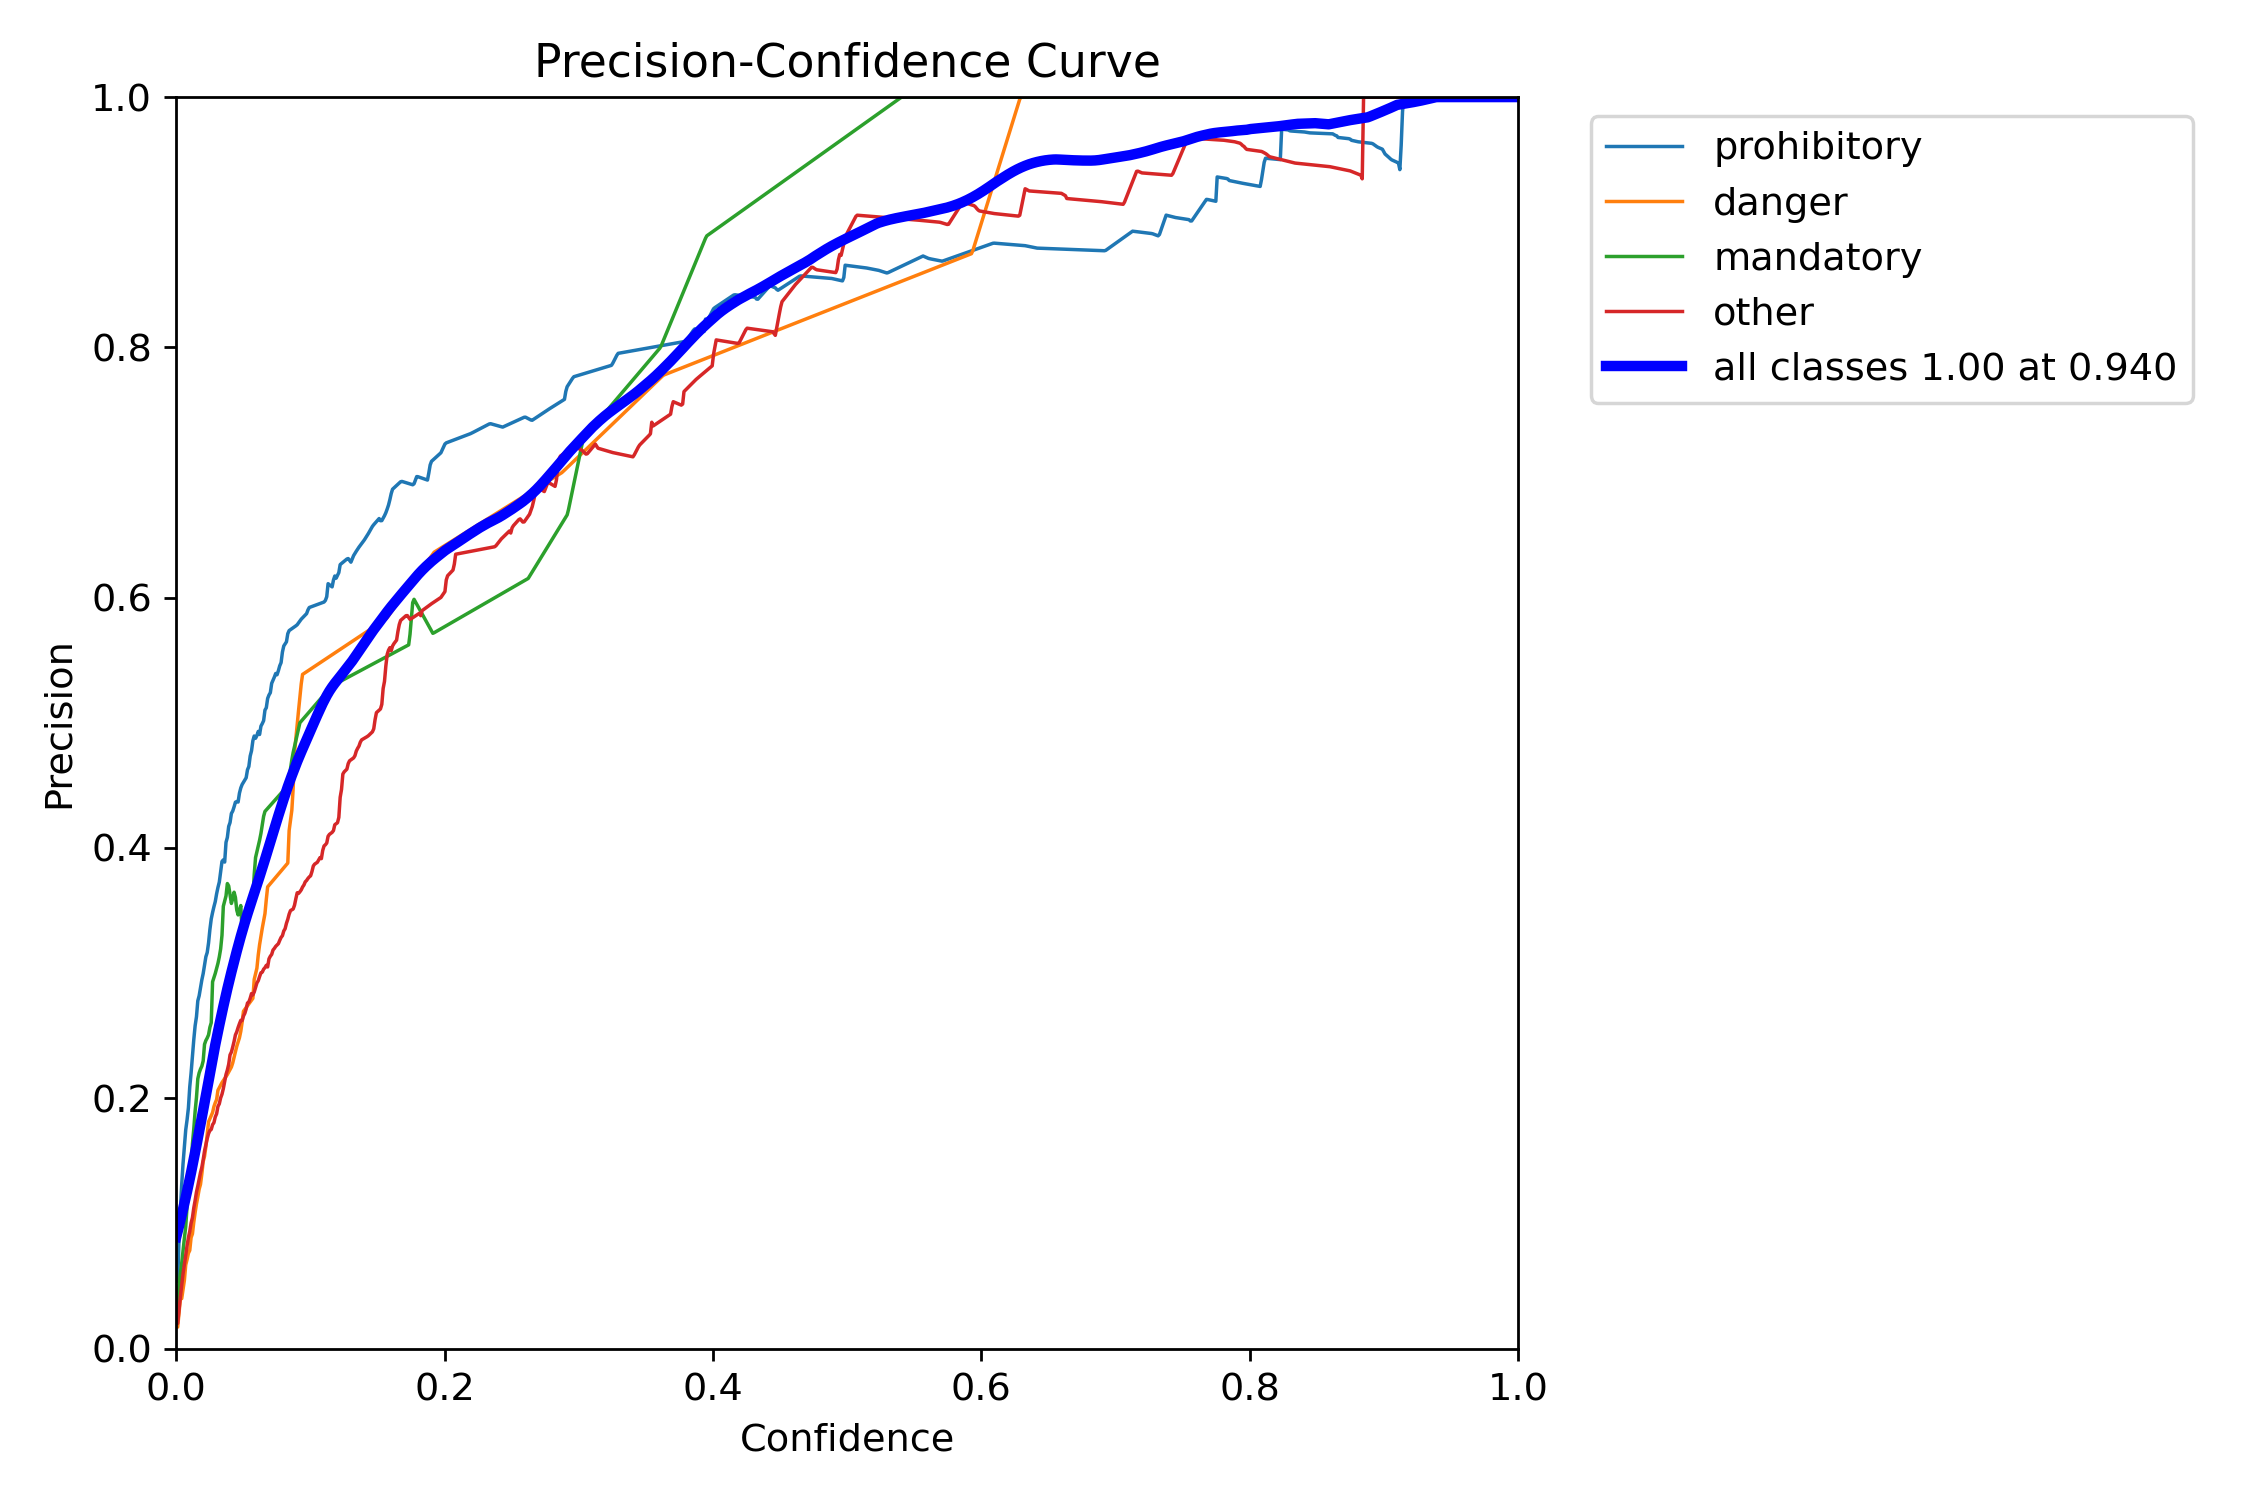
\includegraphics[width=0.9\textwidth]{resources/random cuban P curve.png}
\caption{}
\end{subfigure}
\begin{subfigure}[b]{0.5\textwidth}
\centering
\includegraphics[width=0.9\textwidth]{resources/sim cuban P  curve.png}
\caption{}
\end{subfigure}
\caption{Métricas en el conjunto CTSRD. a) Precisión en el conjunto aleatorio b) Precisión en el conjunto ordenado}
\label{fig:precision random vs precision sim}
\end{figure}

En las gráficas anteriores (figura \ref{fig:precision random vs precision sim}) observamos una leve mejora en la precision de las clases \textbf{Prohibición y Obligación}, además de que se suaviza la curva promedio lo cual sugiere una mayor generalización del modelo.


\begin{figure}[h]
\begin{subfigure}[b]{0.5\textwidth}
\centering
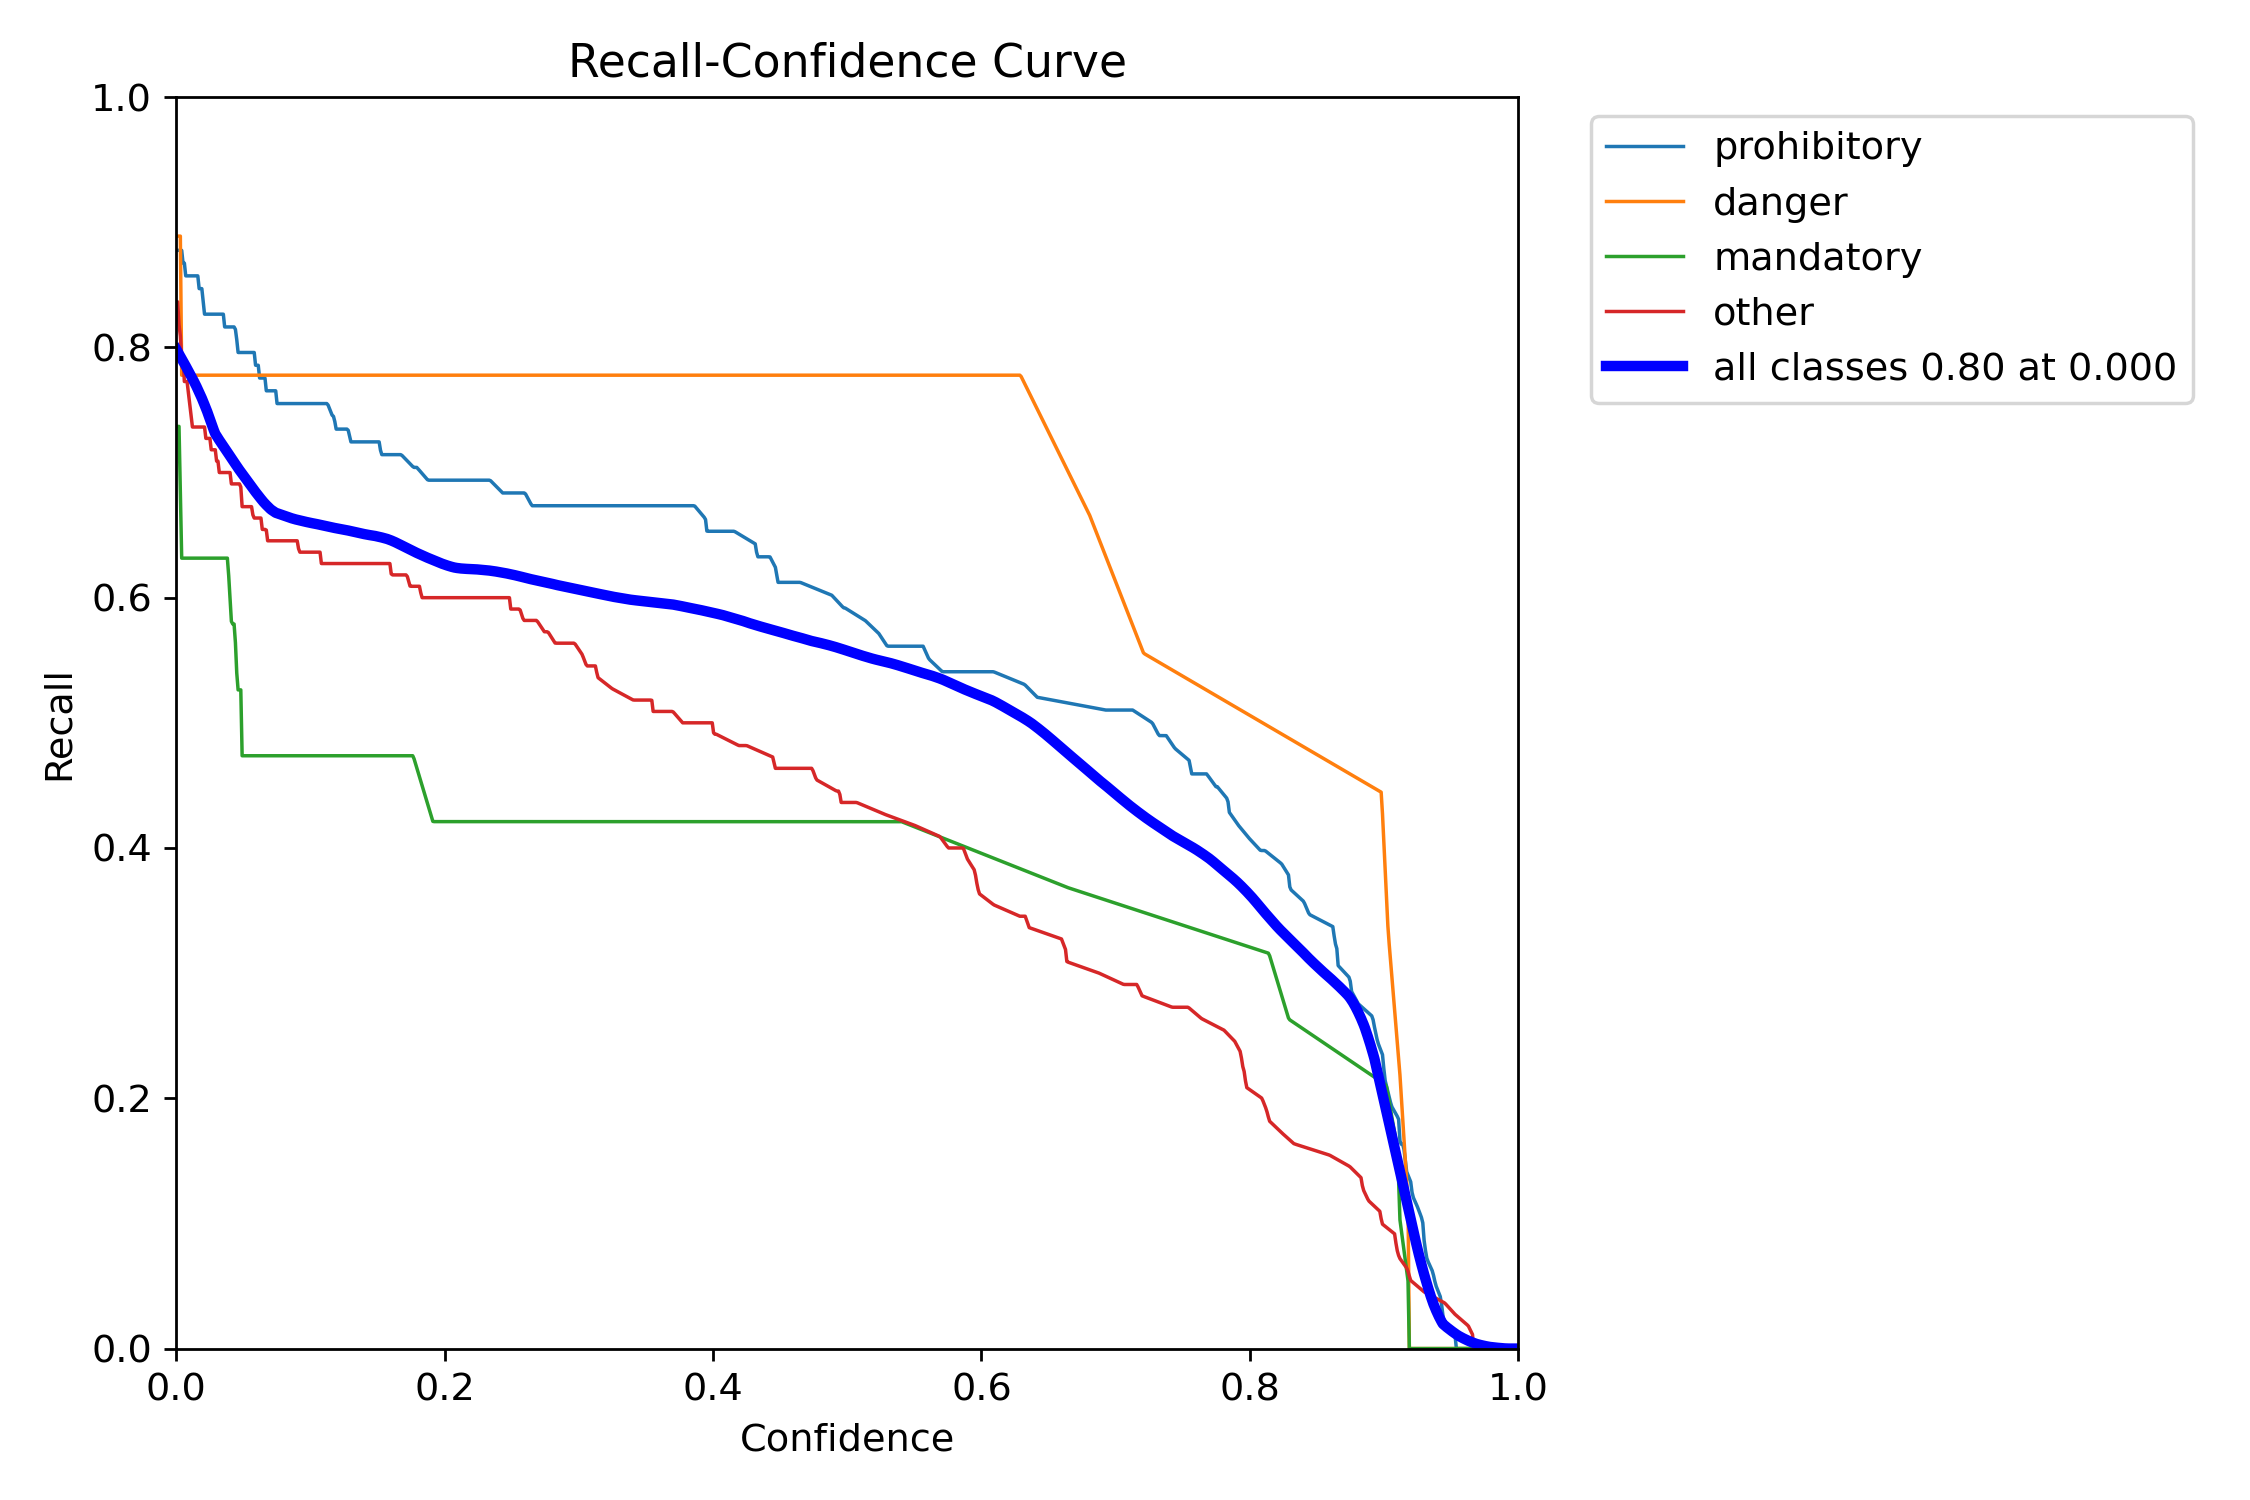
\includegraphics[width=0.9\textwidth]{resources/random cuban R curve.png}
\caption{}
\end{subfigure}
\begin{subfigure}[b]{0.5\textwidth}
\centering
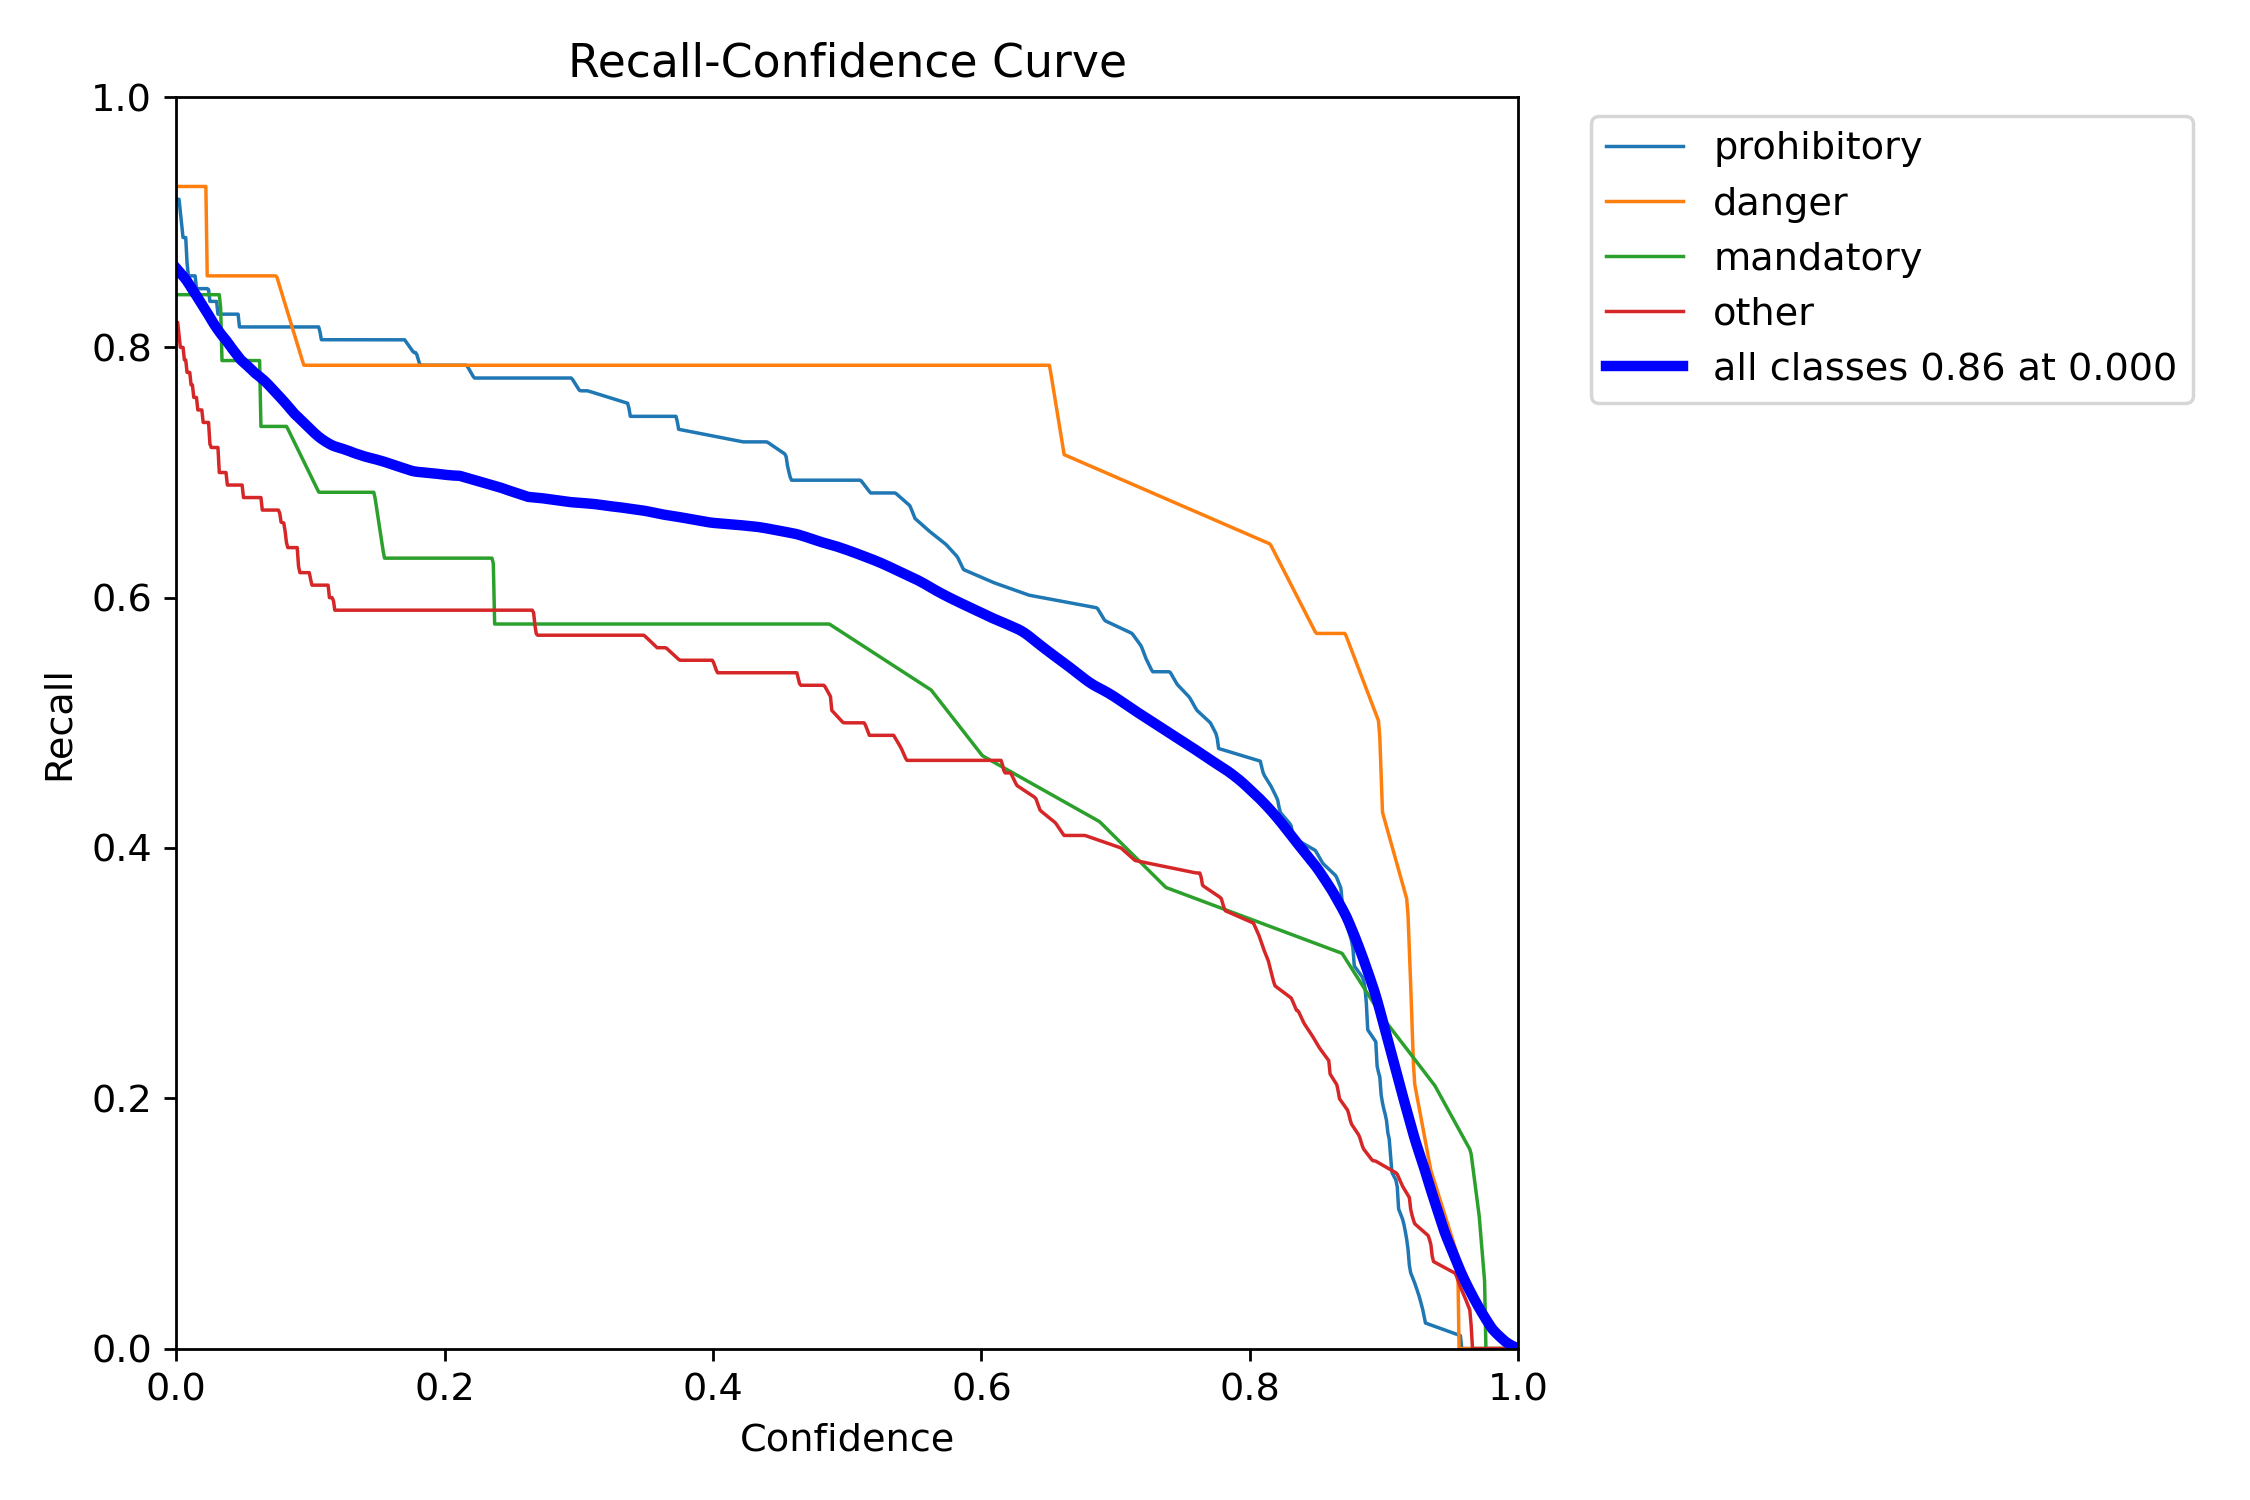
\includegraphics[width=0.9\textwidth]{resources/sim cuban R curve.png}
\caption{}
\end{subfigure}
\caption{Métricas en el conjunto CTSRD. a) Recobrado en el conjunto aleatorio b) Recobrado en el conjunto ordenado}
\label{fig:recall random vs recall sim}
\end{figure}

En las gráficas de recobrado (figura \ref{fig:recall random vs recall sim}), se aprecia una mejora en todas las clases. Esto significa que, después de reorganizar los datos de entrenamiento y validación, el segundo modelo muestra una mayor capacidad para identificar correctamente los casos positivos de cada clase. En otras palabras, el segundo modelo es más efectivo en términos de recobrado, ya que es capaz de encontrar y clasificar correctamente una mayor proporción de verdaderos positivos para todas las categorías evaluadas. Esta mejora en el recobrado sugiere que la nueva organización de los datos ha permitido al modelo aprender patrones más representativos y generalizables, lo cual se refleja en un mejor rendimiento en la detección de todas las clases consideradas.

\begin{figure}[h]
\begin{subfigure}[b]{0.5\textwidth}
\centering
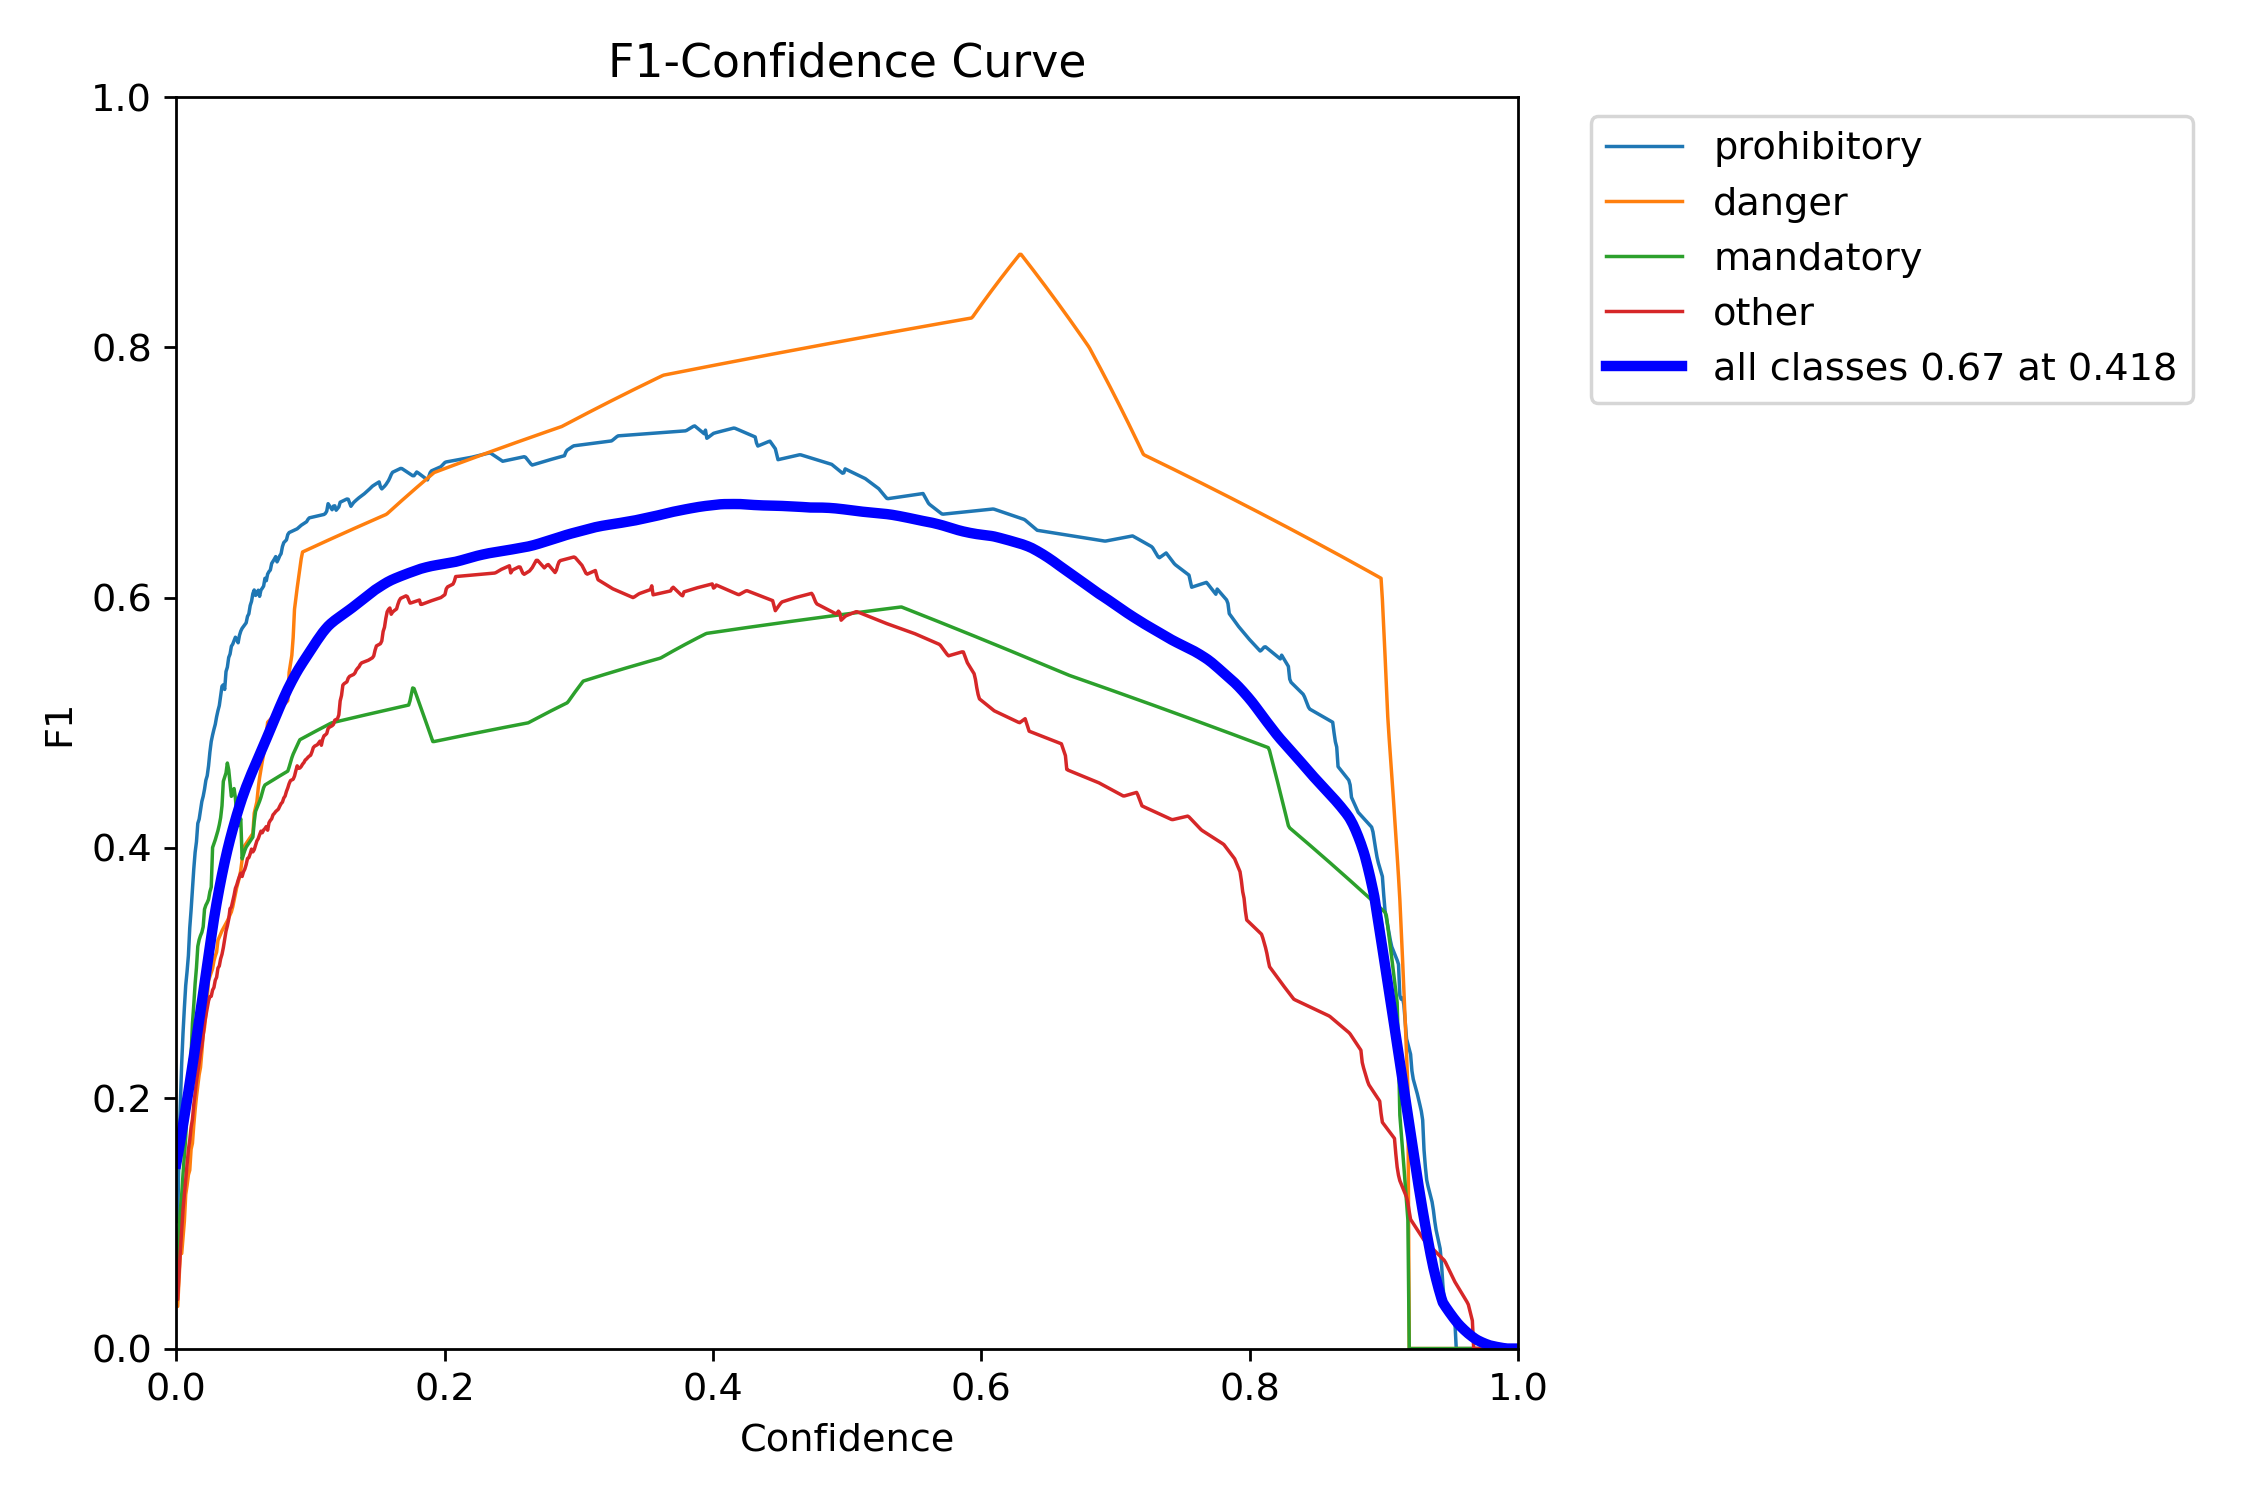
\includegraphics[width=0.9\textwidth]{resources/random cuban F1 curve.png}
\caption{}
\end{subfigure}
\begin{subfigure}[b]{0.5\textwidth}
\centering
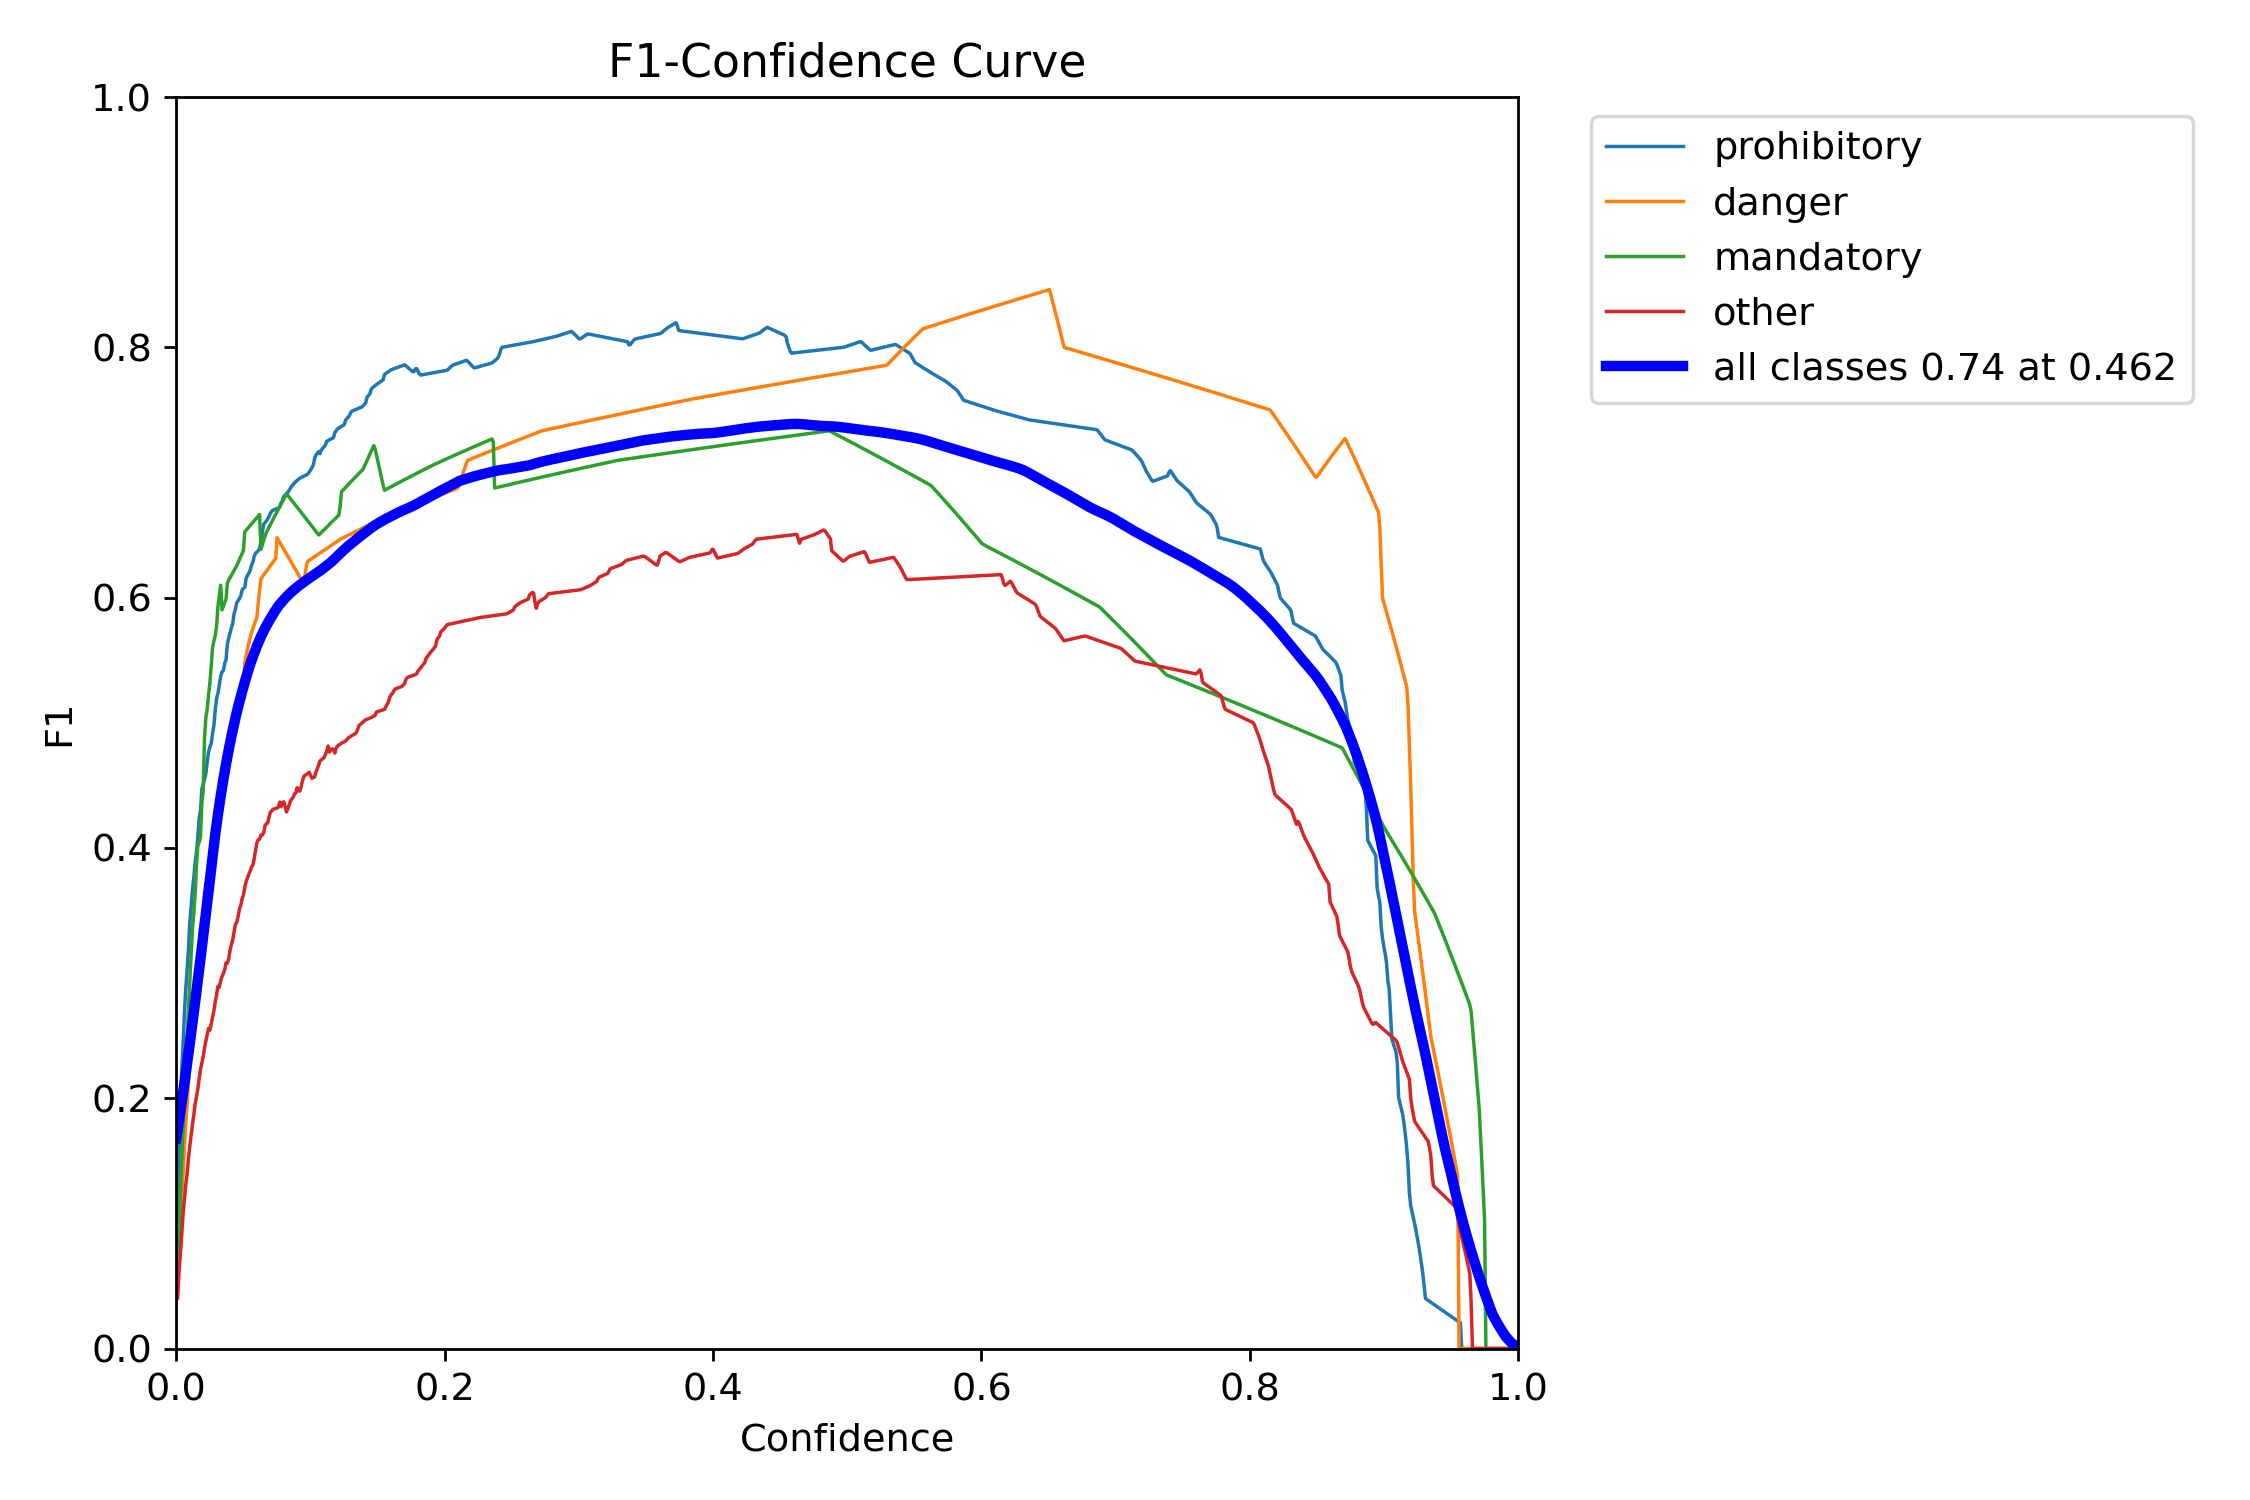
\includegraphics[width=0.9\textwidth]{resources/sim cuban F1 curve.png}
\caption{}
\end{subfigure}
\caption{Métricas en el conjunto CTSRD. a) F1 en el conjunto aleatorio b) F1 en el conjunto ordenado}
\label{fig:f1 random vs f1 sim}
\end{figure}

La mejora en las curvas de F1 (figura \ref{fig:f1 random vs f1 sim}) implica que la reorganización de los datos ha permitido al segundo modelo obtener una representación más efectiva y generalizable de los datos, resultando en un rendimiento superior y más robusto en la clasificación de todas las clases evaluadas.



\begin{figure}[h]
\begin{subfigure}[b]{0.5\textwidth}
\centering
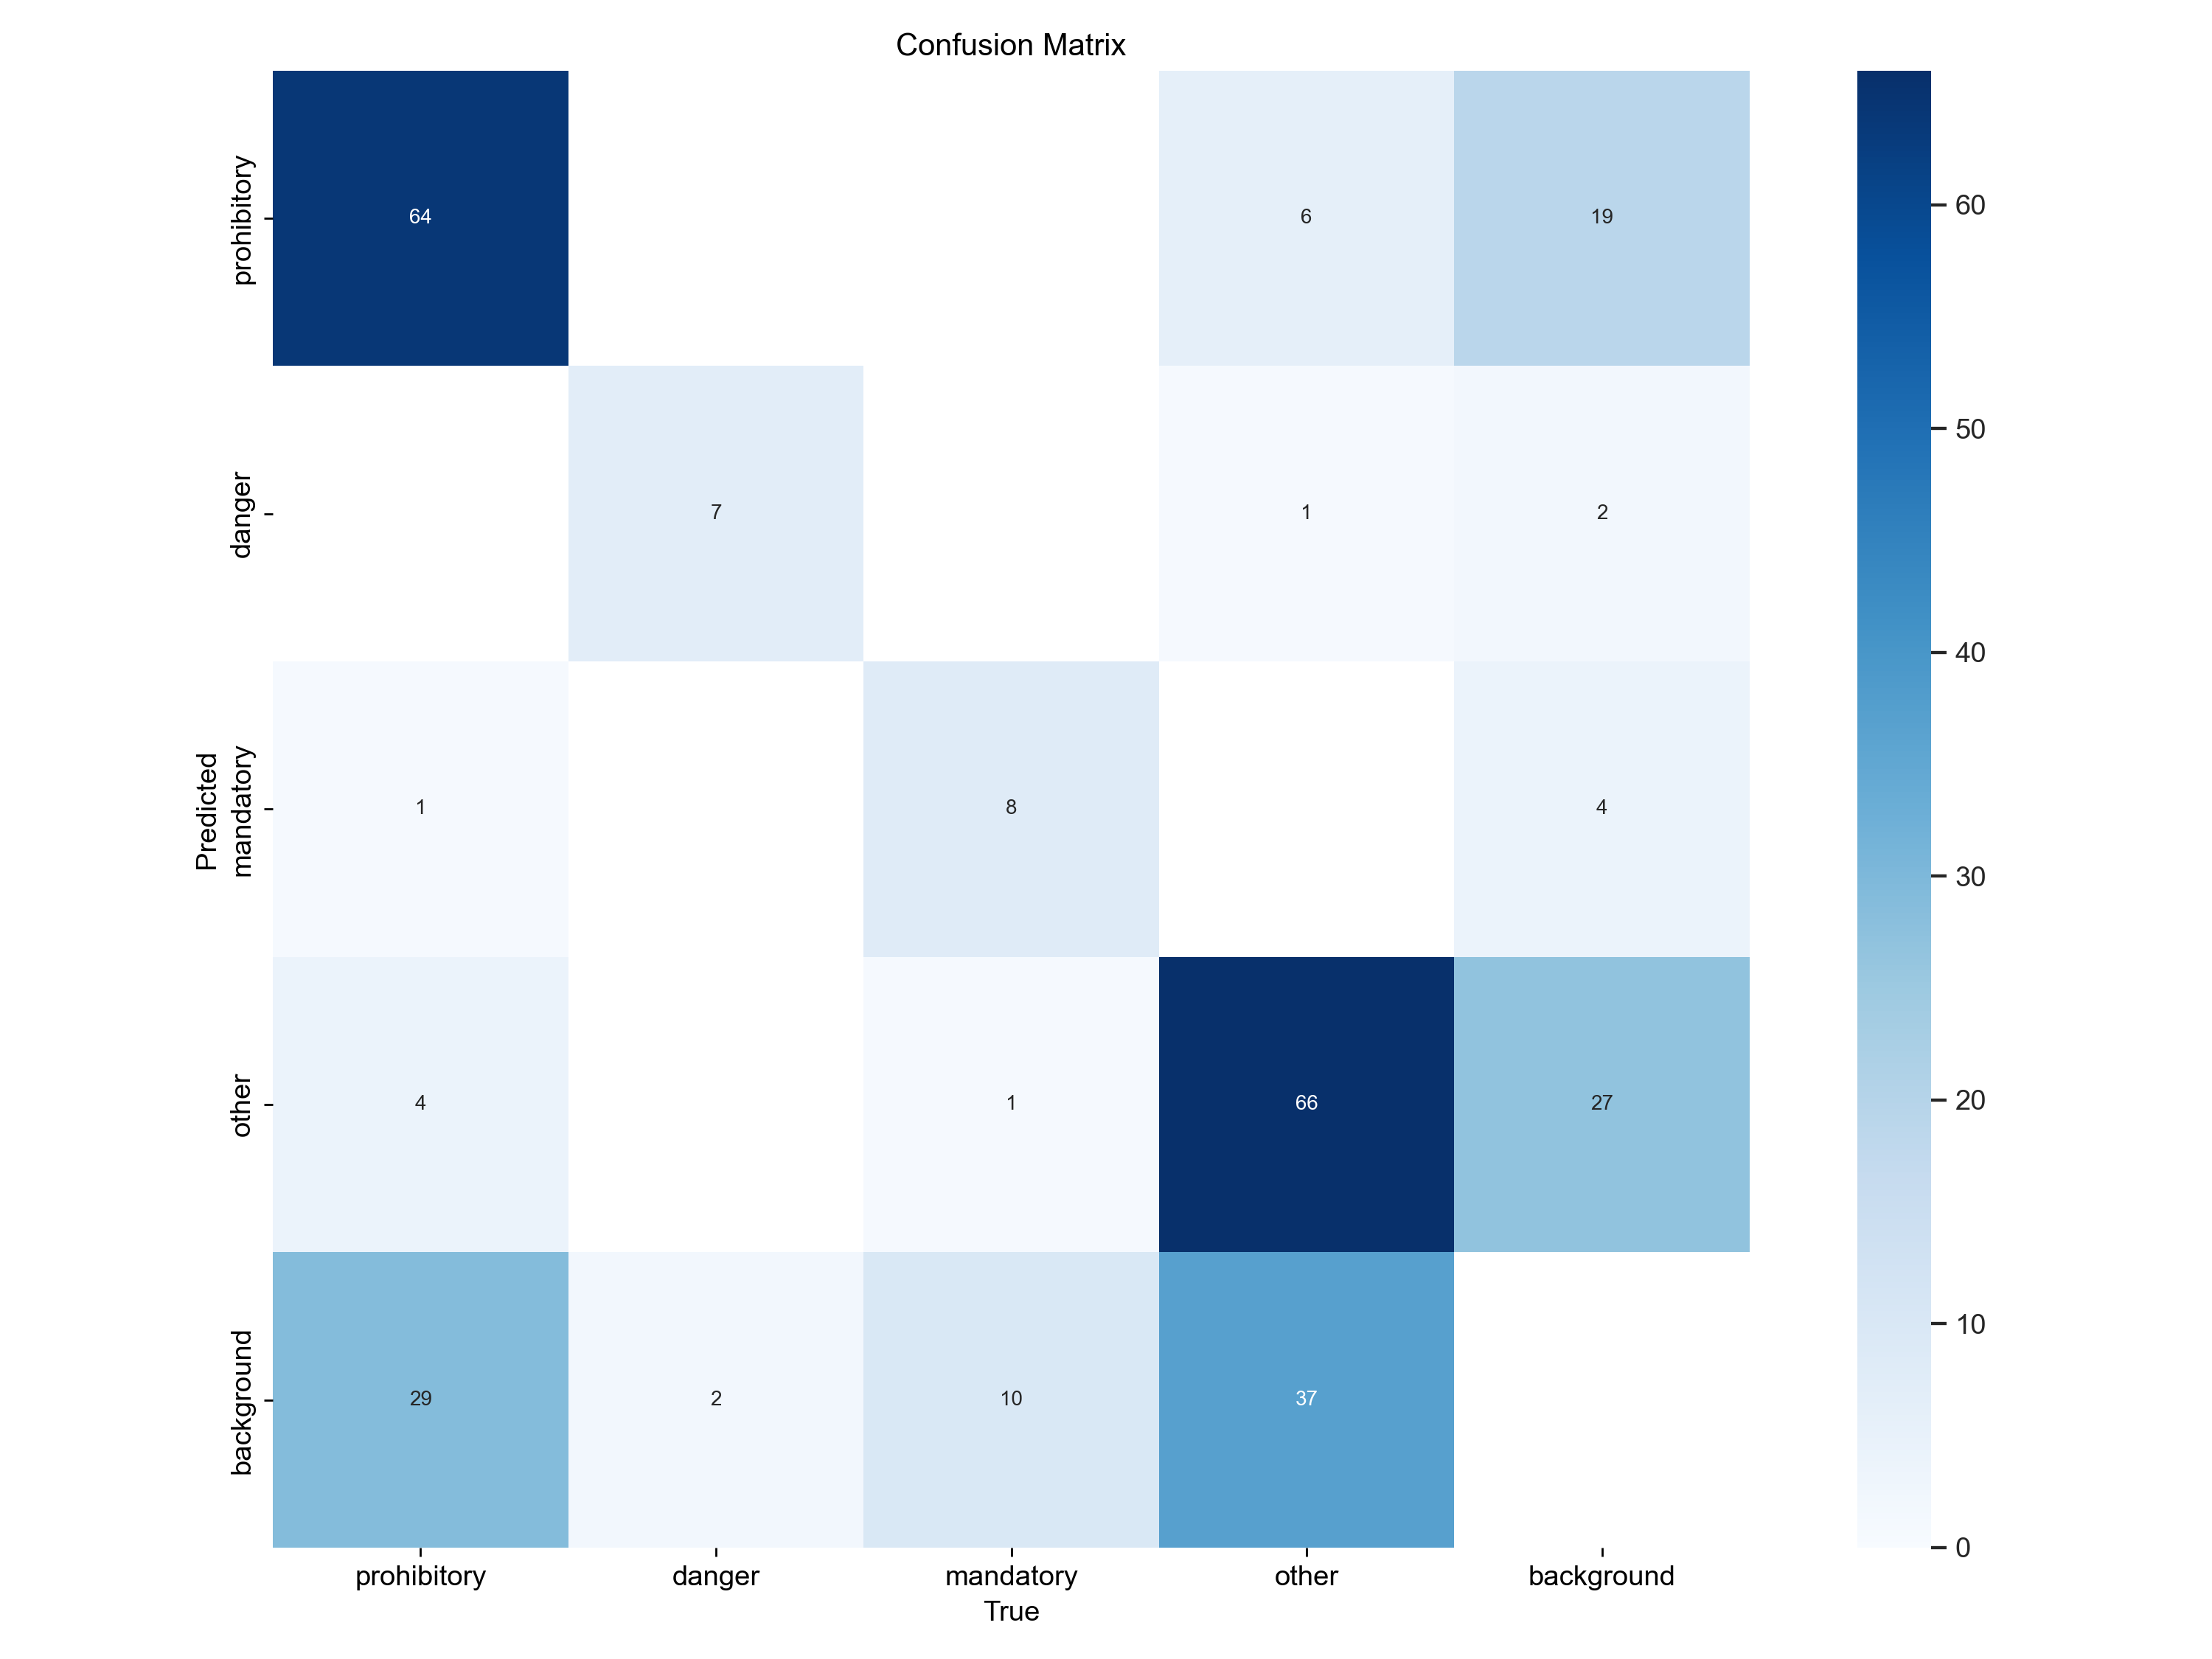
\includegraphics[width=0.9\textwidth]{resources/random cuban confusion matrix.png}
\caption{}
\end{subfigure}
\begin{subfigure}[b]{0.5\textwidth}
\centering
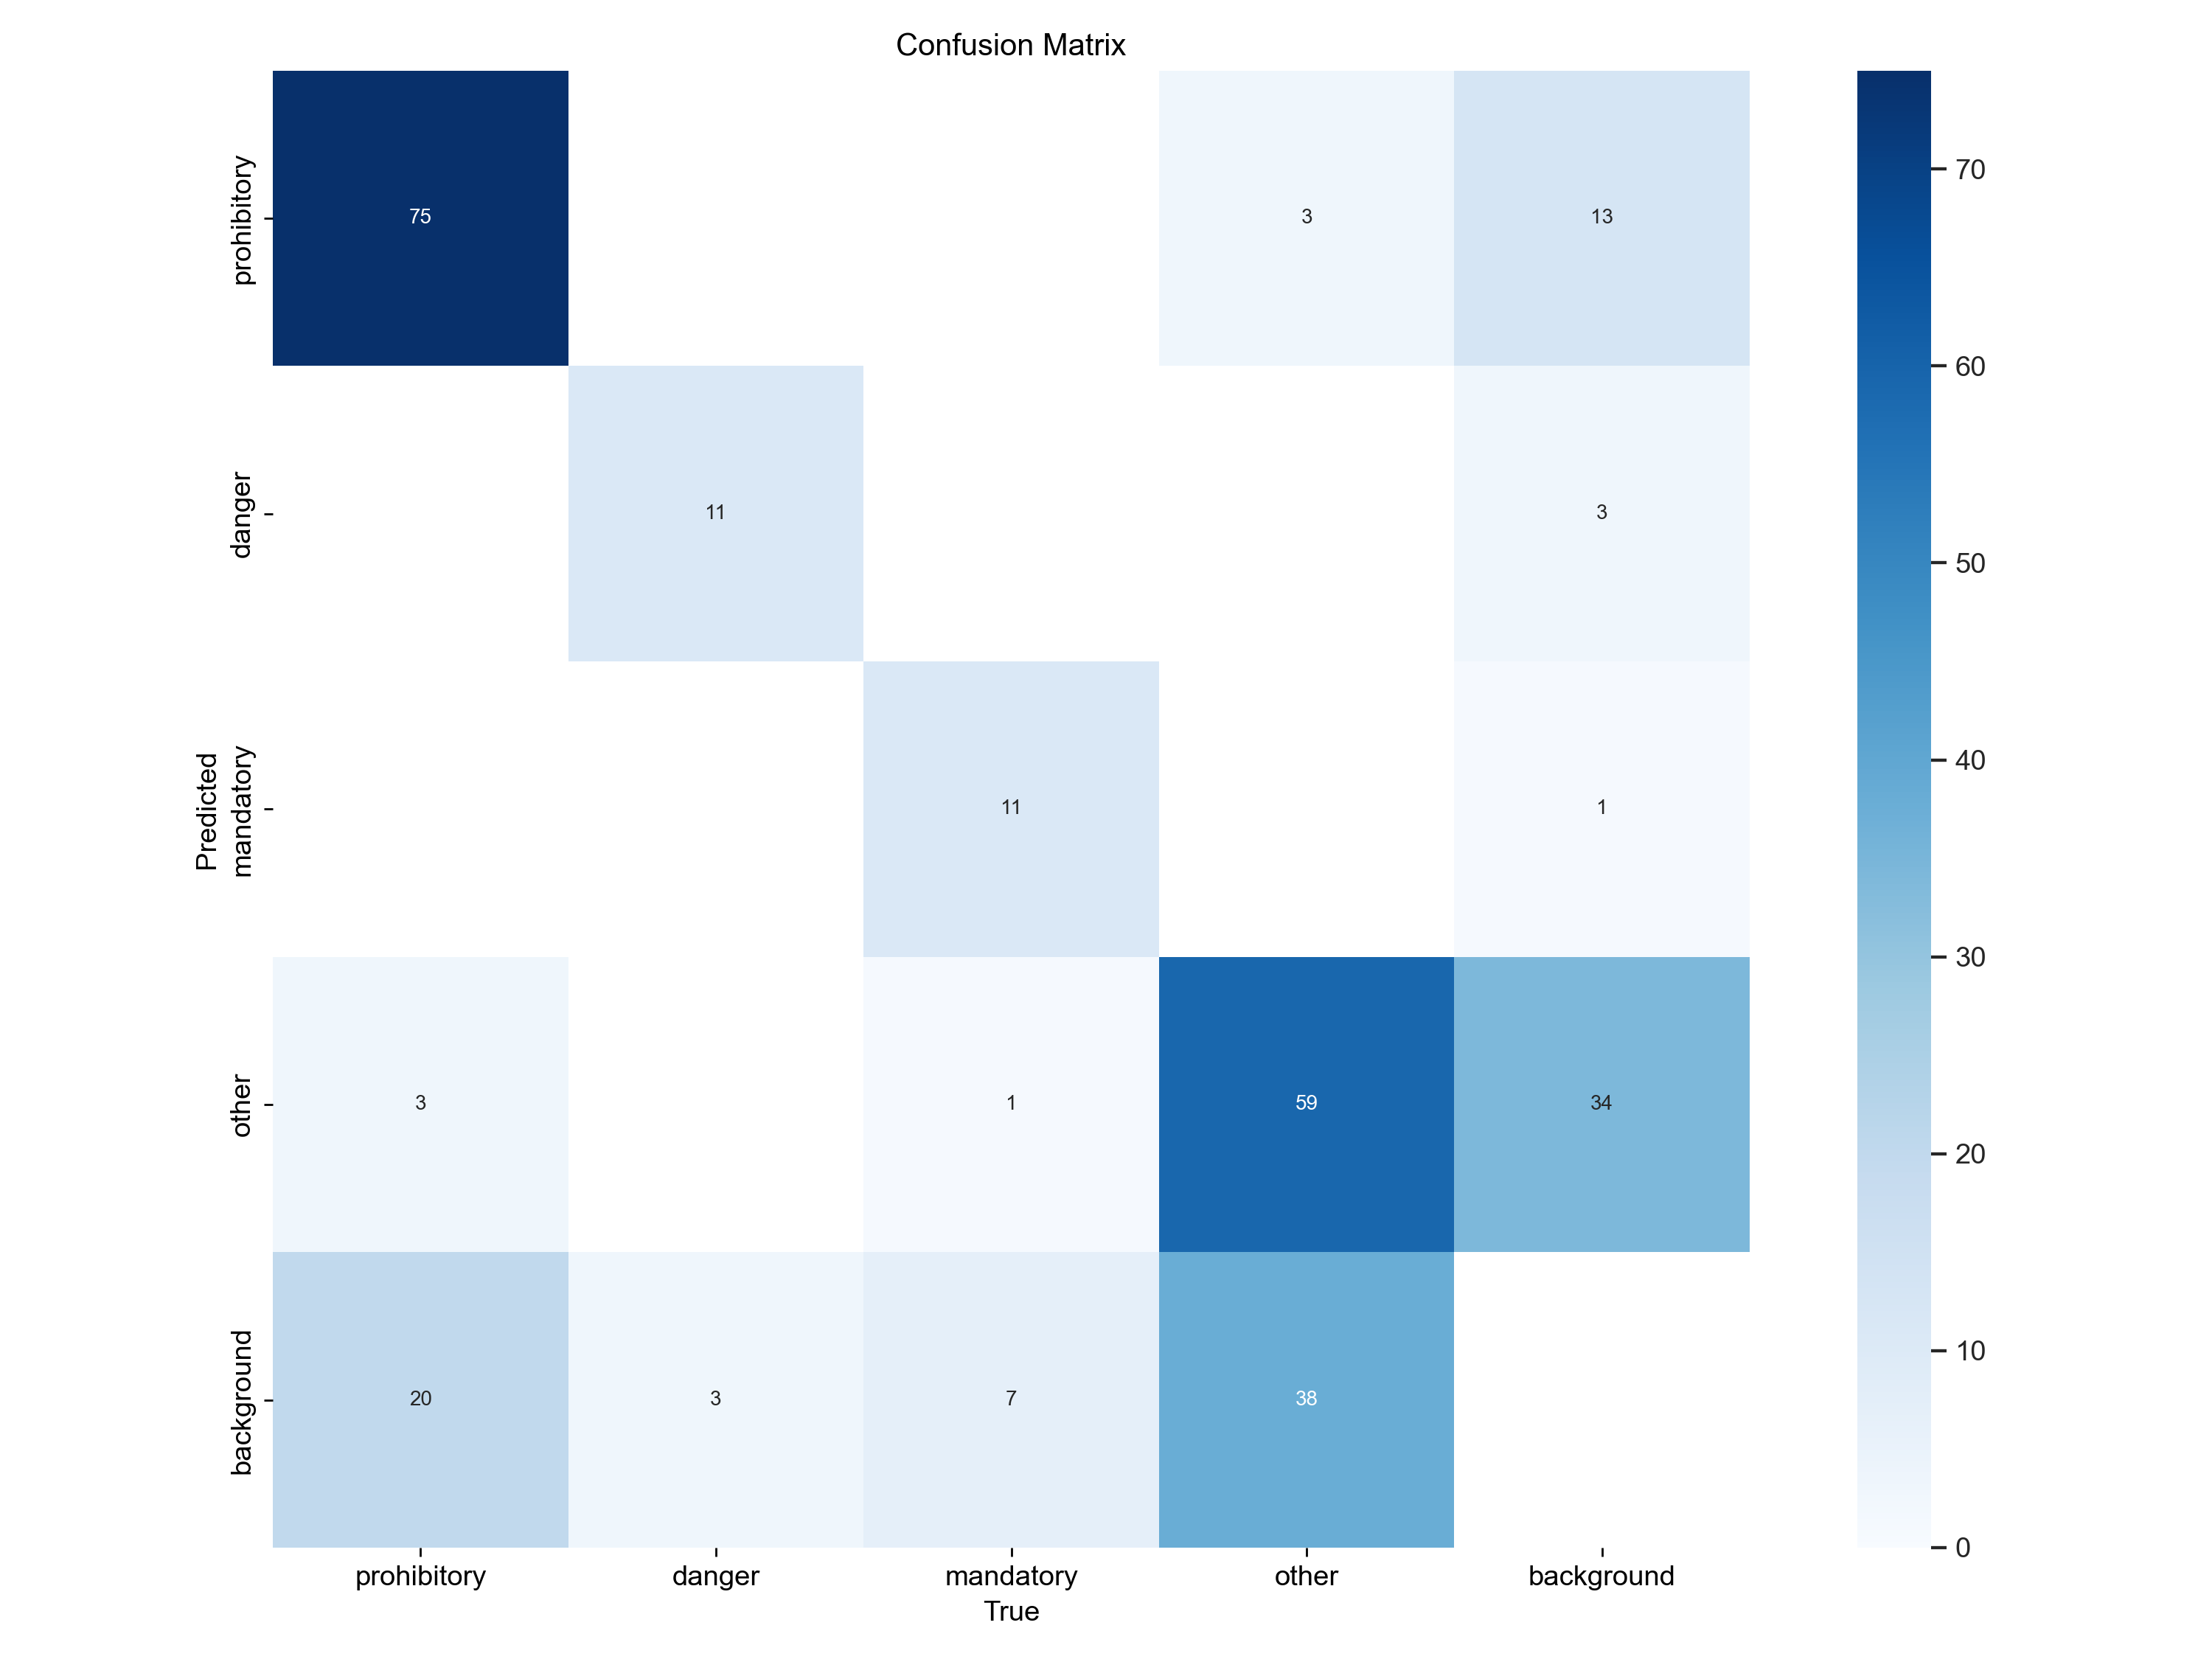
\includegraphics[width=0.9\textwidth]{resources/sim cuban confusion matrix.png}
\caption{}
\end{subfigure}
\caption{Métricas en el conjunto CTSRD. a) Matriz de confusión del conjunto aleatorio b) Matriz de confusión del conjunto ordenado}
\label{fig:confusion random vs confusion sim}
\end{figure}

Como se puede apreciar en la matriz de confusión (figura \ref{fig:confusion random vs confusion sim}), el modelo organizado fue capaz de clasificar e identificar mejor cada señal, llevándolo a generalizar mejor.

Considerando que el modelo descrito reconoce únicamente las cuatro clases de señales de tráfico mencionadas anteriormente, su implementación se sugiere como un complemento para aumentar la atención de conductores inexpertos en la vía. Este sistema puede funcionar eficazmente como una alerta preventiva, especialmente en el caso de señales de prohibición. La tendencia del modelo a detectar señales con mayor frecuencia que a omitirlas, debido a su alta precisión, contribuye a mantener a los conductores en un estado de alerta constante. Esta característica es particularmente beneficiosa para prevenir accidentes, ya que asegura que los conductores sean informados oportunamente sobre la presencia de señales críticas, permitiéndoles tomar las acciones necesarias para evitar situaciones de peligro.

\subsection{Pruebas de campo}

Como parte de las pruebas de campo, hemos acoplado una cámara a un vehículo de forma que grabe el recorrido del mismo por las calles. Tras un análisis estadístico de la distribución de las señales de tránsito en la vía, en diferentes regiones, consideramos óptima la localización de la cámara, a $5/8$ de proporción horizontal, a la altura de la base del parabrisas (figura \ref{fig:windshield}).

\begin{figure}[h]
\centering
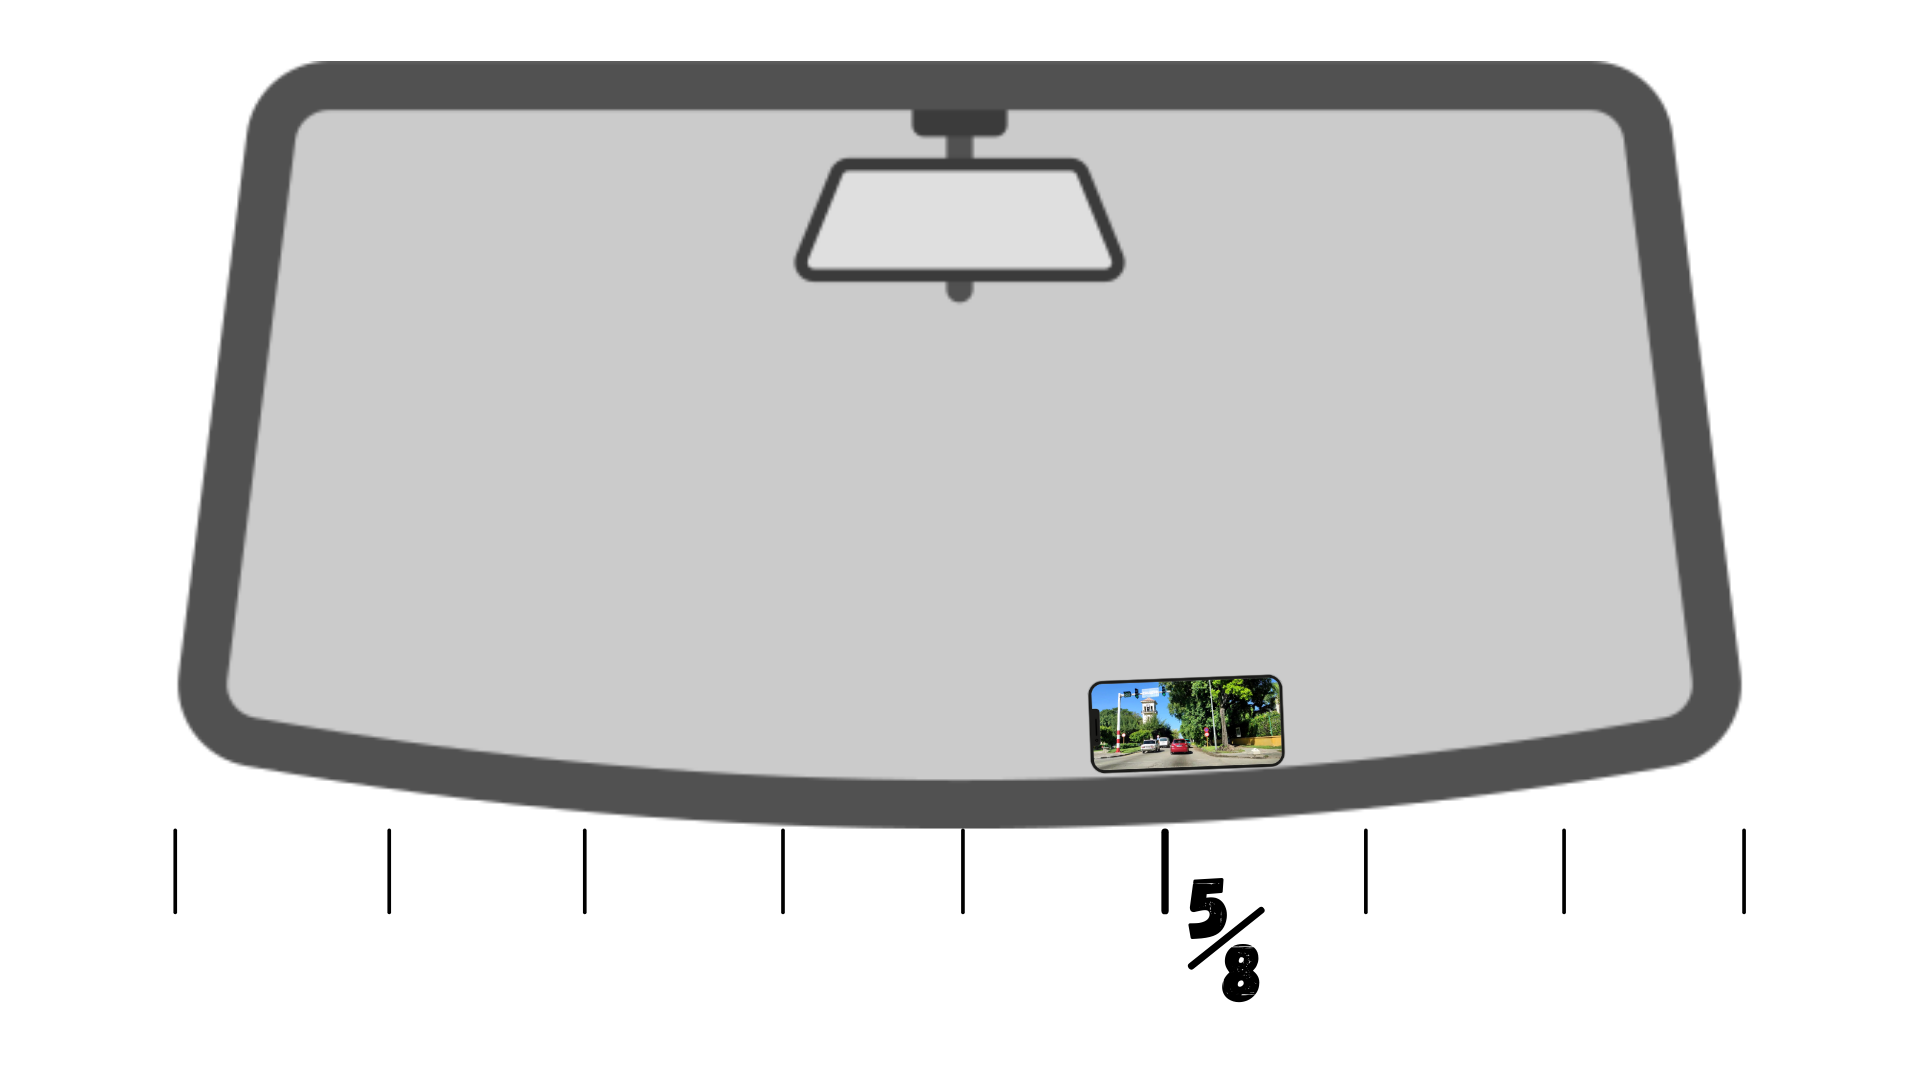
\includegraphics[width=0.9 \textwidth]{resources/windshield.png}
\caption{Localización de la cámara}
\label{fig:windshield}
\end{figure}

La razón de la elección de esta proporción se basa en que la mayoría de las señales de tránsito en carretera se encuentran cercanas al borde derecho de la calle, sin descuidar las que se encuentran en el lado izquierdo; y en menor cantidad en la parte superior de la carretera, junto a semáforos.\\
Dada la necesidad de obtener resultados certeros en las predicciones de las señales, hemos utilizado un valor de confianza del $70\%$. Vale aclarar que como el propósito final de este modelo es en grabaciones en tiempo real, la cantidad de capturas en poco tiempo es alta, por lo que existe una mayor probabilidad de detectar una señal que existe, si en una captura falla.\\
Algunas grabaciones obtenidas han sido postprocesadas por nuestro modelo entrenado, obteniéndose los videos que hubiesen sido detectados en tiempo real.

Con el objetivo de observar mejor el resultado de lo que sería una prueba de campo, hemos provisto el archivo $webcam.py$, que consiste en un script de python que utiliza la webcam integrada en la computadora donde se ejecuta, para obtener predicciones de nuestro modelo en tiempo real.

\begin{tcolorbox}
La frecuencia de capturas depende del procesador de la computadora donde se ejecuta el script.
\end{tcolorbox}
%================================Conclusiones===============================

\section{Conclusiones}
El análisis exhaustivo de señales cubanas mediante técnicas avanzadas de visión computacional revela hallazgos significativos para su aplicación práctica. Los modelos de aprendizaje profundo han demostrado una notable eficacia en la clasificación automática de estas señales, a pesar de desafíos como variaciones en condiciones ambientales y estructurales. Este estudio subraya la viabilidad de implementar sistemas basados en visión computacional para mejorar la seguridad vial y la gestión del tráfico en entornos urbanos cubanos. Sin embargo, se identifica la necesidad urgente de bases de datos anotadas y accesibles, así como la consideración ética en el uso de esta tecnología en espacios públicos. Estos resultados no solo promueven avances en la infraestructura tecnológica local, sino que también abren nuevas perspectivas para la innovación en sistemas de transporte inteligente y conducción autónoma en Cuba.

Se notó, que las imágenes anotadas como \textbf{Otras} son muy variadas en cuanto a sus características visuales, por lo que nuestro modelo no desempeña el mejor papel en la identificación de estas. Una posible solución hubiese sido aumentar los datos anotados con esta clasificación. Otra alternativa pudiese ser dividir esta categoría en las 5 que aparecen en la \textit{Ley 109 del código de seguridad vial}\cite{ref7} asegurando mayores similitudes en su aspecto.

Inicialmente en los objetivos del proyecto estaba hacer un análisis del daño de las señales del tránsito, para así, complementar lo anterior expuesto y proveer un acercamiento al estudio del estado de las señales del tránsito en Cuba. A continuación se ofrecerán una aproximación a posibles soluciones:
\begin{itemize}
 \item{Una solución general hubiese sido, basándonos en aprendizaje supervisado, tener un conjunto de datos con señales dañadas y en buen estado. Esto implicaría la construcción de un nuevo conjunto de datos lo cual es inviable por cuestiones de tiempo y recursos.}
 \item{Una posible aproximación también sería la propuesta por Vanessa Dalborgo et al. \cite{ref11}, ya que en Cuba también hay un problema con señales ocultas por vegetación, para ello, se agregaría una nueva clase al modelo, lo que implicaría una segmentación del conjunto de datos en su totalidad, además de requerir más datos de esta clase que se quiere explotar.}
\item{Por último Bubryur Kim et al. \cite{ref4} proponen un algoritmo para la detección de daño en estructuras de acero, como puentes  y vigas de acero, pero desde una distancia más próxima a las mismas. Se podría utilizar esta propuesta para detectar el daño en las señales de tráfico, por lo anterior expuesto no se puso en practica esta solución.}
\end{itemize}

%========================Glosario===============================

\section{Glosario}
\begin{itemize}
\item{\textbf{Anchor Boxes:} Las anchor boxes son cajas predefinidas de ciertas alturas y anchuras que se utilizan como referencias para predecir las cajas delimitadoras reales alrededor de los objetos.}
\item{\textbf{Backbone:} Se refiere a la red de extracción de características que procesa los datos de entrada en una cierta representación de características. Constituido por las primeras capas del modelo.}
\item{\textbf{Bloques Residuales:} Su idea principal es introducir conexiones de atajo (skip connections) que permiten el flujo de información sin interrupciones a través de la red, saltando una o más capas.}
\item{\textbf{Bottleneck blocks:} Tipo de bloque de convolución que se utiliza para reducir la dimensionalidad de las características intermedias dentro de una red neuronal profunda, y luego expandirlas nuevamente.}
\item{\textbf{Bounding Box:} En la detección de objetos, una bounding box es una caja rectangular que se utiliza para definir la posición y el tamaño del objeto en una imagen.}
\item{\textbf{Épocas de calentamiento:} Técnica utilizada durante el entrenamiento de redes neuronales profundas para suavizar la transición hacia un aprendizaje más agresivo.}
\item{\textbf{Función SoftMax:} La función softmax, o función exponencial normalizada, se emplea para "comprimir" un vector K-dimensional  de valores reales arbitrarios en un vector K-dimensional, de valores reales en el rango [0, 1].}
\item{\textbf{Head:} Parte final de la red que se encarga de realizar la predicción de las salidas deseadas, como las clases de los objetos y sus ubicaciones.}
\item{\textbf{K-Means++:} Es una mejora del algoritmo KMeans estándar. Mejora la inicialización de los centroides para que el algoritmo converja más rápido y alcance una mejor solución final en términos de calidad del clustering.}
\item{\textbf{Transfer Learning:} En lugar de entrenar un modelo desde cero, se aprovecha el conocimiento adquirido por un modelo existente para mejorar la eficiencia y el rendimiento de un nuevo modelo.}
\end{itemize}
%===========================Referencias===================================
\bibliographystyle{plain}
\bibliography{referencias} 
\end{document}



















